%%%%%%%%%%%%%%%%%%%%%%%%%%%%%%%%%%%%%%%%%%%%%%%%%%%%%%%%%%%%%%%%%%%%
%% I, the copyright holder of this work, release this work into the
%% public domain. This applies worldwide. In some countries this may
%% not be legally possible; if so: I grant anyone the right to use
%% this work for any purpose, without any conditions, unless such
%% conditions are required by law.
%%%%%%%%%%%%%%%%%%%%%%%%%%%%%%%%%%%%%%%%%%%%%%%%%%%%%%%%%%%%%%%%%%%%

\documentclass{beamer}
\usetheme[faculty=fss]{fibeamer}
\usepackage[T1]{fontenc}
\usepackage[utf8]{inputenc}
% \usepackage{lmodern}

% \renewcommand\familydefault{\sfdefault}
\usefonttheme[onlymath]{serif}
% \usepackage{newpxtext}
% \usepackage{newpxmath}
% \let\openbox\relax

\usepackage{slantsc}
\usepackage{microtype}
\usepackage[british]{babel}

\usepackage[backend=bibtex, style=trad-abbrv, sorting=none, maxbibnames=3, maxcitenames=2]{biblatex}
\addbibresource{../TFG.bib}
\addbibresource{../TFM.bib}
\addbibresource{../bibliography.bib}
\makeatletter
	\def\blx@maxline{77}
\makeatother

\let\counterwithout\relax
\let\counterwithin\relax

%-----------------------------------------------------------------
%	PDF INFO AND HYPERREF
%-----------------------------------------------------------------
\usepackage{hyperref}
\hypersetup{colorlinks, citecolor=black, filecolor=black, linkcolor=black, urlcolor=black}
\usepackage{cleveref}
	\crefname{section}{\S}{\SS}
	\Crefname{section}{\S}{\SS}
	\crefname{listing}{snippet}{}

\newcommand*{\mytitle}{The influence of sea surface temperature on tropical-cyclone intensity}
\newcommand*{\mysubtitle}{(Provisional Title)}
\newcommand*{\myauthor}{Alfredo Hernández Cavieres}
\newcommand*{\mysupervisora}{Álvaro Corral }
\newcommand*{\mysupervisorb}{Isabel Serra}
\newcommand*{\myuni}{Universitat Autònoma de Barcelona}
\newcommand*{\mydate}{11th July 2018}

\pdfstringdefDisableCommands{\def\and{and }}

\usepackage{hyperxmp}
\usepackage{pdfpages}
\hypersetup{pdfauthor={\myauthor}, pdftitle={\mytitle}}


%-----------------------------------------------------------------
% CUSTOM STYLE FILES
%-----------------------------------------------------------------

% \usepackage{$HOME/LaTeX/style-files/alf-layout-new}
\usepackage{$HOME/LaTeX/style-files/alf-maths}
% \usepackage{$HOME/LaTeX/style-files/alf-misc}
% \usepackage{$HOME/LaTeX/style-files/alf-code}
\usepackage{../alf-code}
% \usepackage{$HOME/LaTeX/style-files/alf-theorems}
% \usepackage{$HOME/LaTeX/style-files/alf-ela}

% \usepackage{enumerate}
% \usepackage[shortlabels]{enumitem}
\usepackage{float}
\usepackage{subfig}
\usepackage{tabularx}
\usepackage{booktabs}
\usepackage{array}
\usepackage{multirow}

\usepackage[linesnumbered,algoruled,vlined]{algorithm2e}

\makeatletter
\def\BState{\State\hskip-\ALG@thistlm}
\makeatother

\newcommand*{\se}[1]{\widehat{\text{se}}(#1)}


%-----------------------------------------------------------------
%% These macros specify information about the presentation
\title{\mytitle}
% \subtitle{Presentation Subtitle}
\author{\myauthor
\\ \footnotesize Supervised by: \mysupervisora \& \mysupervisorb}
%% These additional packages are used within the document:
\usepackage{ragged2e}  % `\justifying` text
\usepackage{booktabs}  % Tables
\usepackage{tabularx}
\usepackage{tikz}      % Diagrams
\usetikzlibrary{calc, shapes, backgrounds}
\usepackage{amsmath, amssymb}
\usepackage{url}       % `\url`s
\usepackage{listings}  % Code listings
\frenchspacing

\begin{document}
	%-----------------------------------------------------------------
%	BODY
%	!TEX root = ./../main.tex
%-----------------------------------------------------------------
% \section{Data background}\label{sec:background}
% \input{./contents/2-data}

%-----------------------------------------------------------------
\section{Introduction}\label{sec:intro}
%-----------------------------------------------------------------
%	INTRODUCTION
%	!TEX root = ./../main.tex
%-----------------------------------------------------------------
% \section{Introduction}\label{sec:intro}
% \todo[inline]{Write the whole thing}
% \begin{itemize}
% 	\item Brief outline of the topic and subtopics being covered in the thesis (referencing sections).
% 	\item Overview of the structure of the code (in terms of how functions are defined in different files and stuff).
% 	\item A rationale as to why the project is an important addition to the current body of knowledge.
% 	\item The main objectives of thesis and a brief overview of how these would be achieved.
% 	\item A hypothesis we want to solve.
% \end{itemize}

For the North Atlantic (N.~Atl.) and Northeast Pacific (E.~Pac.) basin, it has been shown \cite{Corral2010} that the probability distribution of the so-called power-dissipation index ($PDI$, a rough estimation of released energy) is affected by the annual and basin-wide averaged sea surface temperature (SST), displacing towards more extreme values on warm years (high-SST).

As the $PDI$ integrates (cubic) wind speed over tropical-cyclone (TC) lifetime, it is an open question where the $PDI$ increase comes from (higher speed, longer lifetime, or both).

% \todo[inline]{Add finishing paragraph}






%-----------------------------------------------------------------
%	INTRODUCTION: TROPICAL-CYCLONES
%	!TEX root = ./../main.tex
%-----------------------------------------------------------------
\subsection{Tropical-cyclones}\label{sec:intro-hurricanes}
To characterise a tropical-cyclone one needs to define a physically relevant measure of released energy. In \cite{Emanuel1986-bis} \citeauthor{Emanuel1986-bis} showed that in a tropical-cyclone energy dissipation occurs mostly in the atmospheric surface layer, and that the corresponding dissipation rate per unit area, $D$, is
\begin{align}
	D \equiv C_{D} \rho \norm{\va{v}}^{3}
	,
\end{align}
where $C_{D}$ is the surface drag coefficient, $\rho$ is the surface air density, $\norm{\va{v}}$ is the magnitude of the surface wind velocity.

Thus, integrated over the surface area covered by a circularly symmetric tropical-cyclone of radius $r_{0}$ of lifetime $\tau$, the total power dissipated by the storm, $PD$, is given by
\begin{align}
	PD \equiv 2 \pi \int_{0}^{\tau} \int_{0}^{r_{0}} C_{D} \rho \norm{\va{v}}^{3} r \dd{r} \dd{t}
	.
\end{align}

However, as stated in \cite{Emanuel2005}, since the integral in the expression \eqref{eq:pdi} will in practice be dominated by high wind speeds, one can approximate the product $C_{D} \rho$ as a constant and define a simplified power dissipation index ($PDI$) as
\begin{subequations}
\begin{align}\label{eq:pdi}
	PDI \equiv \int_{0}^{\tau} v_{max}^{3} \dd{t}
	.
\end{align}

However, the wind data (as we discuss in~\cref{ssec:hurdat}) is recorded every $\Delta t = \SI{6}{\hour}$. Therefore, we discretise the expression for the $PDI$ using the rectangle method:
\begin{align}\label{eq:pdi-bis}
	PDI = \sum_{t} v_{t}^{3} \Delta t
	,
\end{align}
\end{subequations}
where $v_{t}$ is the maximum sustained surface wind speed at time $t$.

\medskip
Although the $PDI$ is enough to characterise the released energy by a tropical-cyclone, we are interested in the causal relationship between increasing tropical-cyclone $PDI$ and increasing sea surface temperature (SST) proposed by \textcite{Trenberth2005}, as well as the relationship with the lifetime associated to each tropical-cyclone.

\citeauthor{Trenberth2005} states that higher SSTs are associated with increased water vapour in the lower troposphere; both higher SSTs and increased water vapour tend to increase the energy available for atmospheric convection and the energy available to tropical-cyclones as a consequence.

By separating the $PDI$ data by low-SST and high-SST years, we get two similar $PDI$ distributions with one major difference: high-SST years should have a longer right tail on account of having more available energy from the sea (this is explored with more detail in \Cref{ssec:univariate}). For this separation (or classification) process we follow the methodology used by \citeauthor{Corral2010} in~\cite{Corral2010}, which is a variation of the methodology proposed by \citeauthor{Webster2005} in~\cite{Webster2005}.

\sk
To perform this classification we need to calculate first the mean SST of each year $\ev{\text{SST}}$:
\begin{align}
	\ev{\text{SST}} = \sum_{y} \frac{\text{SST}(y)}{Y},
\end{align}
where $\text{SST}(y)$ is the mean SST of the year $y$, and $Y$ is the total number of years studied; as usual, the standard error of this mean, is defined as
\begin{align}\label{eq:sst-sem}
	\se{\text{SST}} = \frac{1}{\sqrt{Y}} \sqrt{ \frac{1}{Y-1} \sum_{y} \qty(\text{SST}(y) - \ev{\text{SST}})^{2} } .
\end{align}

The classification of each year in low-SST and high-SST years is performed depending on whether they are lower or greater than $\ev{\text{SST}}$.

\medskip
If one wishes to consult a thorough technical review article on tropical-cyclone as a thermodynamic system,~\cite{Emanuel2003} by \citeauthor{Emanuel2003} would probably be the best source available.

% To characterise a tropical-cyclone (TC) one needs to define a physically relevant measure of released energy. The released energy of each TC is summarised as
% \begin{equation}\label{eq:pdi}
% 	PDI = \sum_{t} v_{t}^{3} \Delta t .
% \end{equation}
% The raw hurricane best track data (HURDAT2) is provided by the National Hurricane Center. We intentionally limit this study to the satellite era (1966--2016), as it is the most reliable.

% \bigskip
% Then, the hurricane observational data is classified into occurrences in low-SST and high-SST years depending on whether they are lower or greater than
% \begin{equation}
% 	\ev{\text{SST}} = \sum_{y \in Y} \frac{\text{SST}(y)}{Y} ,
% \end{equation}
% where $\text{SST}(y)$ is the mean SST of the year $y$, and $Y$ is the total number of years studied. The SST data (HadISST1) is provided by the Met Office Hadley Centre.

\bigskip
Tropical cyclones are classified into three main groups, based on wind intensity: tropical depressions, tropical storms, and a third group of more intense storms, whose name depends on the region. In particular, in the Northeast Pacific or in the North Atlantic, it is called a hurricane. In \Cref{tab:hurr-class} we can see a detailed classification of the tropical-cyclones studied in this text.
\begin{table}[H]
	\centering
	\begin{tabular}{l c c}
		\toprule
		\toprule
		\multicolumn{1}{c}{Category} & \multicolumn{2}{c}{1--minute sustained winds} \\
		\midrule
		Tropical depression  & $\le \SI{33}{\knot}$      & ($\le \SI{61}{\km/\hour}$) \\
		Tropical storm       & $\SIrange{34}{63}{\knot}$ & ($\SIrange{63}{118}{\km/\hour}$) \\
		Category 1 hurricane & $\SIrange{64}{82}{\knot}$ & ($\SIrange{119}{153}{\km/\hour}$) \\
		Category 2 hurricane & $\SIrange{83}{95}{\knot}$ & ($\SIrange{154}{177}{\km/\hour}$) \\
		Category 3 major hurricane & $\SIrange{96}{112}{\knot}$  & ($\SIrange{178}{208}{\km/\hour}$) \\
		Category 4 major hurricane & $\SIrange{113}{136}{\knot}$ & ($\SIrange{209}{253}{\km/\hour}$) \\
		Category 5 major hurricane & $\ge \SI{137}{\knot}$       & ($\ge \SI{254}{\km/\hour}$) \\
		\bottomrule
	\end{tabular}
	\caption{Tropical-cyclone classification used by the NHC}
	\label{tab:hurr-class}
\end{table}

%-----------------------------------------------------------------
%	INTRODUCTION: HYPOTHESIS AND CONCLUSIONS
%	!TEX root = ./../main.tex
%-----------------------------------------------------------------
\subsection{Hypothesis and conclusions}\label{sec:intro-hypothesis}
The hypothesis is that the $\text{SST}$ does not directly affect the maximum wind speed of a tropical-cyclone: storms of equal lifetime should, in theory, have the same wind speed and $PDI$, and have the same joint distribution:
\begin{align}\label{eq:hypothesis}
	f(Y \mid X = x)_{\text{low}} = f(Y \mid X = x)_{\text{high}} .
\end{align}
The physical reasoning behind this is that once the cyclone is activated, the wind speed should not depend on its underlying $\text{SST}$.

Instead of working with the exact joint
%bivariate log-normal
distributions $f$, we study the expected value of the distributions:
\begin{align}
	E(Y \mid X = x )_{\text{low}} = E(Y \mid X = x )_{\text{high}},
\end{align}
where $E(Y \mid X = x )$ is estimated by performing a \emph{ordinary least squares} (OLS) regression analysis on the data sets.

\bigskip
The results show a remarkable correlation in the joint distribution of lifetime and $PDI$. By considering this joint distribution a bivariate lognormal distribution we perform a linear regression analysis of the logarithmic variables. Statistical testing, by means of a permutation test, shows that there is no significant difference between the regression coefficient estimates for low-SST years and high-SST years.

This gives a strong evidence in favour to the fact that this relation does not significantly depend on the SST. In other words, the wind speed of a tropical cyclone of a given lifetime will be the same (within statistical fluctuations) in cold and warm years.

% \medskip
% Our conclusions are compatible with the view of tropical cyclones as an activation process, in which, once the event has started, its intensity is kept in critical balance between attenuation and intensification (and so, higher SST does not trigger more intensification).

%-----------------------------------------------------------------
%	INTRODUCTION: OUTLINE
%	!TEX root = ./../main.tex
%-----------------------------------------------------------------
\subsection{Outline}
In essence, our methodology consists in comparing the low-SST and high-SST hurricane occurrences distributions to discern any statistical difference between both.

Firstly, in \Cref{sec:distribution-analysis}, for each basin we explore the joint distributions of $PDI$ and storm lifetime and compare low-SST and high-SST years by studying the expected value of the marginal distributions.

For comparing the two populations obtained after separating the hurricane occurrences by low-SST and high-SST years, in \Cref{sec:statistics-intro} we propose a null hypothesis and test statistics, which are evaluated in \Cref{sec:reg-analysis-data}.

\medskip
To be able to fit a linear regression model using ordinary least squares, some critical assumptions on the residual errors need to hold. These are tested in \Cref{ssec:testing-assumptions} using diagnostic plots and specific statistical tests designed to test each assumption.

After finding that some of these assumptions do not actually hold, in \Cref{sec:bootstrap} we perform a resampling of the observations using a bootstrap method to provide a more accurate and robust regression analysis than the one provided by the ordinary least squares method. Then the same test statistics are evaluated using the bootstrapped coefficient estimates.

\medskip
The only issue with these test statistics, is that it is hard to tell from theory if they are too big to reject the null hypothesis. It is for this reason that in \Cref{sec:perm-test} we propose a permutation test to assess the statistical significance of evidence against (or in favour of) the tested hypothesis that there is no difference in the evolution of a tropical-cyclone once it is activated, regardless of the SST.

\medskip
To answer why the increase of tropical-cyclone lifetime with SST triggers an increase in wind speed as a by-product, as a first approach in \Cref{sec:geographical-analysis} we perform an exploratory analysis of the geographical properties of the tropical-cyclones, such as genesis and death location of the storms, as well as their path length. Our results show that the longer lifetimes for high-SST are mainly due to a shift to South-East of the tropical-cyclones genesis point.



%-----------------------------------------------------------------
\section{Background}\label{sec:background-theory}
%-----------------------------------------------------------------
%	BACKGROUND: REGRESSION THEORY
%	!TEX root = ./../main.tex
%-----------------------------------------------------------------
\subsection{Simple linear regression}\label{sec:simple-regression}
\nocite{James2006} \nocite{Dalgaard2008}

Suppose that there is a quantitative \emph{response}, or \emph{dependent variable}, $Y$ and a \emph{predictor}, or \emph{independent variable}, $X$. It is assumed that there is some kind of \emph{true} relationship between $Y$ and $X$, which can be written as
\begin{align}
	Y = f(X) + \epsilon,
\end{align}
where $f$ is an fixed but unknown function of $X$, and $\epsilon$ is a random \emph{error term} assumed independent and $\mc{N}(0, \, \sigma^{2})$, i.e., distributed normally  with mean $\mu = 0$ and variance $\sigma^{2}$. %This homogeneity of variance $\sigma^{2}$ is also called \emph{homoscedasticity}.

If $f$ is to be approximated by a linear function, then this relationship can be written as
\begin{align}\label{eq:lm-model}
	Y = \beta_{0} + \beta_{1} X + \epsilon.
\end{align}

Here $\beta_{0}$ is the \emph{intercept} term, that is, the expected value of $Y(X = 0)$, and $\beta_{1}$ is the \emph{slope}, the average increase in $Y$ associated with a one-unit increase in $X$. The error term $\epsilon$ takes into account that (i) the true relationship is probably not exactly linear, (ii) there may be other variables that cause variation in $Y$, and (iii) there may be measurement error.

\bigskip
The simple linear regression helps building, or fitting, a statistical model for predicting, or estimating, the dependent variable $Y$ based on the dependent variable $X$.

%-----------------------------------------------------------------
\subsection{Estimation of the coefficients}\label{sec:lm-coefs}

In practice, the coefficients $\beta_{0}$ and $\beta_{1}$, as well as
% the \emph{residual standard error}
$\sigma^{2}$ are unknown. The most common method to find the coefficients is the \emph{least squares regression} or \emph{ordinary least squares} (OLS).

Suppose the studied data set $(X, Y)$ consists of $n$ observation pairs
\begin{align*}
	(x_{1} , y_{1}), (x_{2} , y_{2}), \dots, (x_{i} , y_{i}), \dots , (x_{n} , y_{n}).
\end{align*}

Let $\hat{y}_{i} = \hat{\beta}_{0} + \hat{\beta}_{1} x_{i}$ be the prediction for $Y$ based on the $i$-th value of $X$, where $\hat{\beta}_{0}$ and $\hat{\beta}_{1}$ are the coefficients estimates. Then, $\epsilon_{i} = y_{i} - \hat{y}_{i}$ is the $i$-th \emph{residual} of the linear model. One can define the \emph{residual sum of squares} (RSS) as:
\begin{align}
	\text{RSS} = \sum_{i=1}^{n} \qty(y_{i} - \hat{y}_{i})^{2} = \sum_{i=1}^{n} \qty(y_{i} - (\hat{\beta}_{0} + \hat{\beta}_{1} x_{i}))^{2}.
\end{align}

The OLS approach finds the coefficients $\hat{\beta}_{0}$ and $\hat{\beta}_{1}$ that minimise the RSS:
\begin{subequations}\label{eq:min-pdv}
\begin{align}
	\pdv{\text{RSS}}{\hat{\beta}_{0}} &= - 2 \sum_{i=1}^{n} (y_{i} - (\hat{\beta}_{0} + \hat{\beta}_{1} x_{i})) = 0, \label{eq:min-a} \\
	\pdv{\text{RSS}}{\hat{\beta}_{1}} &= - 2 \sum_{i=1}^{n} x_{i} (y_{i} - (\hat{\beta}_{0} + \hat{\beta}_{1} x_{i})) = 0. \label{eq:min-b}
\end{align}
\end{subequations}

From equation \eqref{eq:min-a}, we can show that the minimiser intercept is
\begin{subequations}\label{eq:regression-coefs}
\begin{align}
	\hat{\beta}_{0} = \bar{y} - \hat{\beta}_{1} \bar{x},
\end{align}
where $\bar{x}$ and $\bar{y}$ are the sample means of $X$ and $Y$, respectively:
\begin{align*}
	\bar{x} = \frac{1}{n} \sum_{i=1}^{n} x_{i} \qc
	\bar{y} = \frac{1}{n} \sum_{i=1}^{n} y_{i}.
\end{align*}

On the other hand, replacing $\hat{\beta}_{0}$ by $\bar{y} - \hat{\beta}_{1} \bar{x}$ in equation \eqref{eq:min-b}, we find that the minimiser slope is
\begin{align}
	\hat{\beta}_{1} = \frac{\sum_{i=1}^{n} \qty(x_{i} - \bar{x}) \qty(y_{i} - \bar{y})}{\sum_{i=1}^{n} \qty(x_{i} - \bar{x})^{2}} . %= \frac{s_{x,y}}{s_{x}^{2}},
\end{align}
\end{subequations}

%-----------------------------------------------------------------
\subsection{Accuracy of the coefficients: standard errors}
% \subsection{Accuracy of the coefficients: confidence intervals}
If we estimate $\hat{\beta}_{0}$ and $\hat{\beta}_{1}$ on the basis of a particular subset of $Y$, then the estimates will not be exactly equal to $\beta_{0}$ and $\beta_{1}$. But if we could average the estimates obtained over a huge number of data sets from $Y$, then the average of these estimates would be exactly equal to $\beta_{0}$ and $\beta_{1}$. This means that the coefficient estimates given by \eqref{eq:regression-coefs} are \emph{unbiased}, or in other words, that the estimators do not systematically over- or under-estimate the true value of the coefficients.

The question, then, arises: how close $\hat{\beta}_{0}$ and $\hat{\beta}_{1}$ are to the true values $\beta_{0}$ and $\beta_{1}$. In general, to answer this, we need to compute the variances or \emph{standard errors} associated with $\beta_{0}$ and $\beta_{1}$:
\begin{subequations}
\begin{align}
	\se{\hat{\beta}_{0}} &= \sqrt{ \sigma^{2} \qty(\frac{1}{n} + \frac{ \bar{x}^{2} }{ \sum_{i=1}^{n} \qty(x_{i} - \bar{x})^{2} } ) }
	,
	\\
	\se{\hat{\beta}_{1}}  &= \sqrt{ \frac{ \sigma^{2} }{ \sum_{i=1}^{n} \qty(x_{i} - \bar{x})^{2} } }
	.
\end{align}
\end{subequations}

In general, $\sigma^{2}$ is not known, but can be estimated from the data. The estimate
of $\sigma$ is known as the \emph{residual standard error} ($\text{RSE}$), and is given by:
\begin{align}
	\hat{\sigma} = \text{RSE} = \sqrt{\frac{\text{RSS}}{n - 2}}.
\end{align}

Note that the assumption here, and the OLS as a whole, is that the variance $\sigma^{2}$ is homogeneous, or in other, words $\operatorname{Var}(\epsilon_{i}) = \sigma^{2},\, \forall i$. This property is called \emph{homoscedasticity}.

The term $n-2$ comes from the fact that the determination of the coefficients is subject to the constraints \eqref{eq:min-a} and \eqref{eq:min-b}. That leaves $n-2$ degrees of freedom for the values of $y_{i}$ in order to determine the linear model exactly.

\bigskip
The estimates $\hat{\beta}_{0}$ and $\hat{\beta}_{1}$ are normally distributed and optimal if the errors $\epsilon_{i}$ are normally distributed. They are often approximately normal for other error distributions, but they are not robust to gross non-normality of errors or to outlying response values.

In \cref{sec:reg-analysis-issues} we will discuss with more detail some techniques to study the normality and homoscedasticity of the random errors. %will be discussed with more detail in .%, as well as a method to improve the linear model in case of non-normality.


% \bigskip
% Standard errors can be used to compute confidence intervals. A $(1 - \theta)$
% confidence interval is defined as a range of values such that with $(1 - \theta)$ interval probability, the range will contain the true unknown value of the parameter. The range is defined in terms of lower and upper limits computed from the sample of data. For linear regression, the \SI{95}{\percent} ($\theta = 0.05$, called \emph{significance level}\footnote{Usually the significance level is represented by $\alpha$, but to avoid confusions we have decided upon a different notation.}) confidence intervals for $\beta_{0}$ and $\beta_{1}$ approximately take the form:
% \begin{align}\label{eq:ci-coefs}
% 	\hat{\beta}_{0} \pm t_{\theta/2, n-2} \cdot \se{\hat{\beta}_{0}}
% 	\qc
% 	\hat{\beta}_{1} \pm t_{\theta/2, n-2} \cdot \se{\hat{\beta}_{1}}
% 	,
% \end{align}
% where $t_{\theta/2, n-2}$ is the $t$ statistic or $t$-value corresponding to the $(\theta/2)$th percentile of a two-sided Student's $t$-distribution on $n-2$ degrees of freedom. On the limit $n \to \infty$, for $(1 - \theta) = 0.95$, then $t_{n-2} = 1.96$. For this reason, for large values of $n$ the \SI{95}{\percent} confidence intervals for the coefficient estimates can be rewritten as
% \begin{align}\tag{\ref{eq:ci-coefs} bis}
% 	\hat{\beta}_{0} \pm 1.96 \cdot \se{\hat{\beta}_{0}}
% 	\qc
% 	\hat{\beta}_{1} \pm 1.96 \cdot \se{\hat{\beta}_{1}}
% 	.
% \end{align}


% Fitted lines are often presented with uncertainty bands around them. If there are many observations, the bands will be quite narrow, reflecting a well-determined line, i.e. well estimated $\beta_{0}$ and $\beta_{1}$. These bands often show a marked curvature since the line is better determined near the centre of the point cloud, as shown in \Cref{fig:conf-intervals}.
% \begin{figure}[H]
% 	\centering
% 	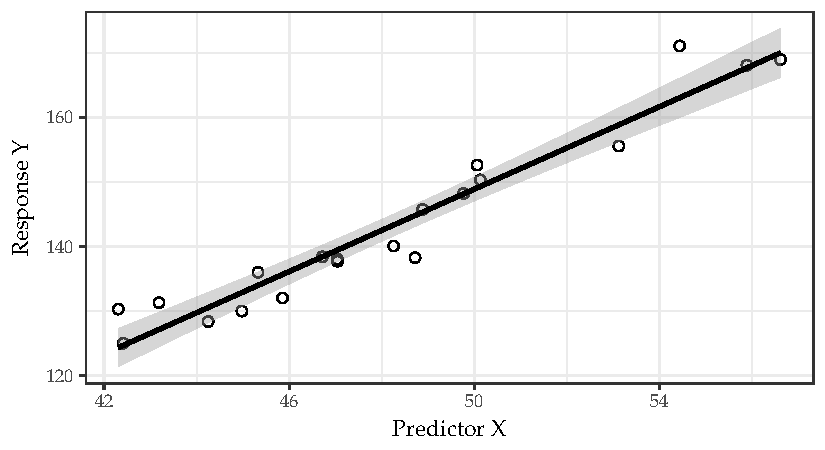
\includegraphics[width=0.9\textwidth]{./images/ci-example}
% 	\caption{\SI{95}{\percent} confidence interval for a simulated linear model $Y = - 10 + 3 X + \epsilon$, with $\sigma^{2} = 5$}
% 	\label{fig:conf-intervals}
% \end{figure}

%-----------------------------------------------------------------
\subsection{Accuracy of the model: \texorpdfstring{$R^{2}$}{R-squared} and correlation}
The goodness of a fit can be assessed by measuring the \emph{correlation coefficient} $r$, or in the more general context of \emph{multiple linear regression}, the $R^{2}$ statistic. In this section we will introduce the mathematical expressions of both coefficients and show their equivalence when studying the simple linear regression:
\begin{align}\label{eq:R2-r2}
	R^{2} = r^{2}.
\end{align}

\subsubsection{\texorpdfstring{$R^{2}$}{R-squared} statistic}
The statistic $R^{2}$ is used in the context of multiple linear regression, and particularly the simple linear regression, and is called the \emph{squared multiple correlation coefficient}, or simply \emph{R-squared}.

\bigskip
The $R^{2}$ statistic is given by
\begin{align}
	R^{2} %= \frac{\text{ESS}}{\text{TSS}}
	 	  = \frac{\text{TSS} - \text{RSS}}{\text{TSS}}
		  = 1 - \frac{\text{RSS}}{\text{TSS}}
	\qc 0 \leq R^{2} \leq 1,
\end{align}
where TSS is the \emph{total sum of squares}:
\begin{align}
	\text{TSS} = \sum_{i=1}^{n} \qty(y_{i} - \bar{y}_{i})^{2}.
\end{align}

TSS measures the total variance in the response $Y$, and can be thought of as the amount of variability inherent in the response before the regression is performed. In contrast, RSS measures the amount of variability that is left unexplained after performing the regression. Hence, $\text{TSS} - \text{RSS}$ measures the amount of variability in the response that is \emph{explained} by the regression model:
\begin{align}
	\text{ESS} = \text{TSS} - \text{RSS} = \sum_{i=1}^{n} \qty(\hat{y}_{i} - \bar{y}_{i})^{2},
\end{align}
and $R^{2}$ measures the proportion of variability in $Y$ that can be explained using $X$ as the predictor.

An $R^{2}$ statistic that is close to 1 indicates that a large proportion of the variability in the response has been explained by the regression model. A number near 0 indicates that the regression did not explain much of the variability in the response; this might occur because the linear model is wrong, the inherent error $\sigma^{2}$ is high, or both.

\subsubsection{Correlation coefficient}
A correlation coefficient is a symmetric, scale-invariant measure of association between two random variables, $X$ and $Y$. It ranges from $-1$ to $+1$, where the extremes indicate perfect correlation and 0 means no correlation. The sign is negative when large values of one variable are associated with small values of the other and positive if both variables tend to be large or small simultaneously. The most common correlation coefficient is the Pearson correlation.

\bigskip
The Pearson correlation, or Pearson's $r$, is rooted in the bivariate normal distribution $f(X, Y)$ (described in \cref{sec:bvln-distribution})
% \todo{Keep reference?}
where the theoretical correlation describes the contour ellipses for the density function. If both variables are scaled to have a variance of 1, then a correlation of zero corresponds to circular contours, whereas the ellipses become narrower and finally collapse into a line segment as the correlation approaches $\pm 1$, which is why sometimes $r$ is called the \emph{linear correlation}.

\bigskip
The empirical correlation coefficient is given by
\begin{align}
	r = \operatorname{Cor}(X,Y)
	  = \frac{\operatorname{Cov}(X,Y)}{\sqrt{\operatorname{Var}(X) \operatorname{Var}(Y) }}
	  =\frac{ \sum_{i=1}^{n} \qty(x_{i} - \bar{x}) \qty(y_{i} - \bar{y}) }{ \sqrt{\sum_{i=1}^{n} \qty(x_{i} - \bar{x})^{2} \sum_{i=1}^{n} \qty(y_{i} - \bar{y})^{2} } }
	  % \qc
	  ,\,\,\,
	  -1 \le r \le 1.
\end{align}

It can be shown that in the context of simple linear regression, the square of the correlation coefficient $r^{2}$ and the $R^{2}$ statistic are identical:
\begin{sproof}
\begin{flalign*}
	R^{2} &= 1 - \frac{\text{RSS}}{\text{TSS}}
		  = 1 - \frac{\sum_{i=1}^{n} \qty(y_{i} - \hat{y}_{i})^{2}}{\sum_{i=1}^{n} \qty(y_{i} - \bar{y}_{i})^{2}}
		  = 1 - \frac{\sum_{i=1}^{n} \qty(y_{i} - \hat{y}_{i})^{2}}{\sum_{i=1}^{n} \qty(y_{i} - \bar{y}_{i})^{2}}
		  = 1 - \frac{\sum_{i=1}^{n} \qty( y_{i} - (\hat{\beta}_{0} + \hat{\beta}_{1} x_{i}) )^{2}}{\sum_{i=1}^{n} \qty(y_{i} - \bar{y}_{i})^{2}}
		  & \\
		  &
		  =1 - \frac{\sum_{i=1}^{n} \qty( y_{i} - (\bar{y} + \hat{\beta}_{1} \bar{x} + \hat{\beta}_{1} x_{i}) )^{2}}{\sum_{i=1}^{n} \qty(y_{i} - \bar{y}_{i})^{2}}
		  = 1 - \frac{\sum_{i=1}^{n} \qty( y_{i} - \bar{y} - \hat{\beta}_{1} \qty(x_{i} - \bar{x}) )^{2}}{\sum_{i=1}^{n} \qty(y_{i} - \bar{y}_{i})^{2}}
		  \\
		  &
		  = 1 - \frac{\sum_{i=1}^{n} \qty(y_{i} - \bar{y})^{2} + \hat{\beta}_{1}^{2} \sum_{i=1}^{n} \qty(x_{i} - \bar{x})^{2} - 2 \hat{\beta}_{1} \sum_{i=1}^{n} \qty(x_{i} - \bar{x}) \qty(y_{i} - \bar{y}) }{\sum_{i=1}^{n} \qty(y_{i} - \bar{y}_{i})^{2}}
		  \\
		  &
		  = \frac{2 \hat{\beta}_{1} \sum_{i=1}^{n} \qty(x_{i} - \bar{x}) \qty(y_{i} - \bar{y}) - \hat{\beta}_{1}^{2} \sum_{i=1}^{n} \qty(x_{i} - \bar{x})^{2} }{\sum_{i=1}^{n} \qty(y_{i} - \bar{y}_{i})^{2}}
		  \\
		  &
		  = \frac{ 2 \dfrac{\sum_{i=1}^{n} \qty(x_{i} - \bar{x}) \qty(y_{i} - \bar{y})}{\sum_{i=1}^{n} \qty(x_{i} - \bar{x})^{2}} \sum_{i=1}^{n} \qty(x_{i} - \bar{x}) \qty(y_{i} - \hat{y}) - \qty( \dfrac{ \sum_{i=1}^{n} \qty(x_{i} - \bar{x}) \qty(y_{i} - \bar{y})}{\sum_{i=1}^{n} \qty(x_{i} - \bar{x})^{2}} )^{2} \sum_{i=1}^{n} \qty(x_{i} - \bar{x})^{2} }{\sum_{i=1}^{n} \qty(y_{i} - \bar{y}_{i})^{2}}
		  \\
		  &
		  %%% = \frac{ 2 \qty( \sum_{i=1}^{n} \qty(x_{i} - \bar{x}) \qty(y_{i} - \bar{y}) )^{2} - \qty( \sum_{i=1}^{n} \qty(x_{i} - \bar{x}) \qty(y_{i} - \bar{y}) )^{2} }{ \sum_{i=1}^{n} \qty(x_{i} - \bar{x})^{2} \sum_{i=1}^{n} \qty(y_{i} - \bar{y})^{2} }
		  = \frac{ \qty( \sum_{i=1}^{n} \qty(x_{i} - \bar{x}) \qty(y_{i} - \bar{y}) )^{2} }{ \sum_{i=1}^{n} \qty(x_{i} - \bar{x})^{2} \sum_{i=1}^{n} \qty(y_{i} - \bar{y})^{2} }
		  = r^{2}. \tag{\ref{eq:R2-r2} bis}
\end{flalign*}
\end{sproof}

\medskip
In simple terms, although they have the same mathematical expression, conceptually $r^{2}$ (and $r$) is an indicator of the strength of the correlation between the variables $X$ and $Y$; while $R^{2}$ is an indicator of the goodness of fit, in the sense of explained variability, of the linear model that predicts the value of $Y$ as a function of $X$ as a causal relationship. Importantly, causality in this context means the direction of causality runs from $X$ to $Y$ and not the other way round.

%-----------------------------------------------------------------
% \vfill
\vspace{0.7cm}
% \subsection{Potential problems with the assumptions}\label{sec:reg-analysis-issues}
\subsection{Regression diagnostics}\label{sec:reg-analysis-issues}

If \eqref{eq:lm-model} holds with homoscedastic random errors $\epsilon_{j}$ and if those random errors are normally distributed, or if the dataset is large, then standard distributional results will be adequate for making inferences with the OLS estimates.
This assumption of homoscedasticity is of big importance in linear regression, as the standard errors, confidence intervals, and hypothesis tests associated with the linear model rely upon it being true.

For this reason, if the errors are grossly non-normal or \emph{heteroscedastic}, meaning that their variances are unequal, then those standard results may not be reliable and a \emph{resampling method} (see \Cref{sec:resampling}) may offer genuine improvement.

\bigskip
% \newpage
To test the normality, independence, and homoscedasticity of the random errors, one can check a few diagnostic plots, which could reveal unexplained patterns in the data by the fitted model. In particular, we will focus on:
\begin{itemize}
	\item Q-Q plot of the residuals.
	\item Residuals vs fitted values plot.
\end{itemize}

\medskip
Additionally, these properties or assumptions on the random errors can be individually tested using some well known statistical hypothesis tests:
\begin{itemize}
	\item Lilliefors test: normality.
	\item Correlation test: independence.
	\item Breusch--Pagan test: homocedasticity.
\end{itemize}

\subsubsection{Q-Q plots}\label{sec:diag-qqplot}
The \emph{Q-Q plot}, or quantile-quantile plot, is a graphical tool to help us assess if a set of data plausibly came from some theoretical distribution such as a normal $\mc{N}(\mu, \, \sigma^{2})$. For example, if we run a statistical analysis that assumes our dependent variable is normally distributed, we can use a \emph{normal Q-Q plot} to check that assumption. It is just a visual check, so it is somewhat subjective, but it can help identify obvious distributional anomalies in the data.

A Q-Q plot is built by taking the sample data, sorting it in ascending order, and then plotting them versus quantiles calculated from the theoretical distribution. In the case of studying the residuals, we expect the data to follow a straight line in the normal Q-Q plot.

\subsubsection{Residuals vs fitted values plots}\label{sec:diag-resid-vs-fitted}
The \emph{residuals vs fitted values plot}, or simply residual plot, is a useful graphical tool to help us assess the homoscedasticity of the residuals or, more generally, if the residuals have non-linear patterns.

A residual plot is built by taking the residuals $\epsilon_{i}$ and plotting them versus the fitted values $\hat{y}_{i}$. The residuals should be centred on zero throughout the range of fitted values, and should be more or less uniformly distributed and have a constant spread throughout the range. The reason behind this is that
\begin{align}
	\operatorname{Cov}(\hat{y}_{i}, \epsilon_{i}) = 0.
\end{align}

One might wonder why do we not just plot the residuals $\epsilon_{i}$ vs the predictors $x_{i}$. Actually, one could plot the residuals vs the predictors, instead of vs the fitted values. However, this plot would be impossible to visualise if we had more than two predictors, so it is of standard practice to look at the residuals vs fitted plot, which is always a 2D plot.

Usually, the residual plot is accompanied by a \emph{locally weighted scatterplot smoothing} (LOWESS) line to help visualise the trend of the residuals. Naturally, under the assumption of normality, the trend should follow a horizontal line centred at $\epsilon = 0$. It is also useful to show the outer quantiles of the residuals to help emphasise and distinguish patterns.

\subsubsection{Lilliefors test}\label{sec:diag-lillie}
The \emph{Lilliefors test}, developed by \citeauthor{Lilliefors1967} (\citeyear{Lilliefors1967}) \cite{Lilliefors1967}, is  a normality test based on the Kolmogorov--Smirnov (KS) test. It is used to test the null hypothesis that data comes from a normally distributed population when the null hypothesis does not specify which normal distribution; in other words, it does not specify the expected value $\mu$ and variance $\sigma^{2}$ of the distribution.

Like most statistical tests, this test of normality defines a criterion and gives its sampling distribution (in this case, a Kolmogorov--Smirnov distribution). When the probability, or $p$-value, associated with the criterion is smaller than a given $\alpha$ significance level, the alternative hypothesis is accepted (i.e., we conclude that the sample does not come from a normal distribution).

A thing to consider with this test is that with small samples, the KS test is underpowered and fails to detect true violations of normality; and with large samples, the KS test may detect violations of normality which are not important for practical purposes~\cite{Razali2010}. For this reason it is important when assessing normality to also look at indicators of the degree of normality such as the Q-Q plot stated previously.

\medskip
In R, the \texttt{nortest} package offers the \texttt{lillie.test()} function to perform the Lilliefors test.

\subsubsection{Correlation test}\label{sec:diag-covtest}
The \emph{Correlation test} is a test based on either Pearson's product-moment correlation, Kendall's rank correlation tau, or Spearman's rank correlation rho. It is used to test the null hypothesis that the correlation between paired samples (in this case, $\epsilon$ and $\hat{Y}$) is zero.

The three methods use different measures of correlation, all in the range $[-1, 1]$ with $0$ indicating no correlation. The most used method is Pearson's product-moment correlation, in which the test statistic is based on Pearson's product moment correlation coefficient $r = \operatorname{Cor}(\epsilon, \hat{Y})$ and follows a Student's $t$-distribution on $n-2$ degrees of freedom.

\medskip
In R, the \texttt{stats} package offers the \texttt{cor.test()} function to perform the Lilliefors test.

\subsubsection{Breusch--Pagan test}\label{sec:diag-bptest}
The \emph{Breusch--Pagan test}, developed by \citeauthor{Breusch1979} (\citeyear{Breusch1979}) \cite{Breusch1979}, is a test used in regression analysis to test for homoscedasticity. It is used to test the null hypothesis that residuals are homoscedastic.

The null hypothesis is that the residual variances are all equal, while the alternative hypothesis is that the residual variances are a multiplicative function of one or more variables. To do this, the test fits a linear regression model to the residuals of a linear regression model (by default the same explanatory variables are taken as in the main regression model) and rejects if too much of the variance is explained by the additional constructed explanatory variables.

\medskip
In R, the \texttt{lmtest} package offers the \texttt{bptest()} function to perform the Breusch--Pagan test.

% \subsubsection{Goldfeld--Quandt test}
% The \emph{Goldfeld--Quandt test} is a test used in regression analysis to test for homoscedasticity. It compares variances of two subgroups; one set of high values and one set of low values. If the variances $\sigma^{2}_{1}$ and $\sigma^{2}_{2}$ differ, the test rejects the null hypothesis that the variances of the errors are not constant.

% Although Goldfeld and Quandt described two types of test in their paper (parametric and non-parametric), the term \emph{Quandt Goldfeld test} usually means the parametric test. The assumption for the test is that the data is normally distributed.

% \medskip
% In R, the \texttt{lmtest} package offers the \texttt{gqtest()} function to perform the Goldfeld-–Quandt test.

\bigskip
\begin{example}
	Let us consider the three different simulated models depicted in \Cref{fig:models-example}. For each of the models, the random error has been built under a different assumption: (a) homoscedasticity, (b) heteroscedasticity, and (c) non-normality.

	For a moment let us forget we know the models behind the data and let us see what we can infer purely from the data, which is generally the case when dealing with real data.

	\begin{figure}[H]
		\centering
		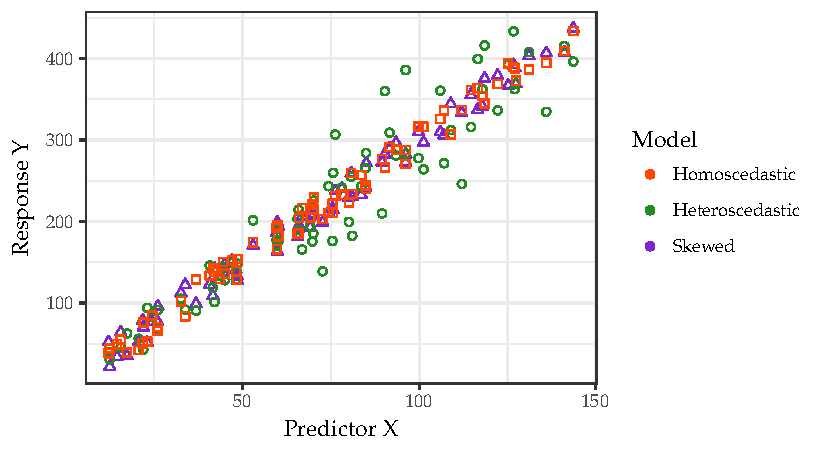
\includegraphics[width=0.8\textwidth]{./images/models-example}
		\caption{Three simulated models of 75 observations each with different response $Y$ in which it would seem appropriate to fit a linear model using OLS}
		\label{fig:models-example}
	\end{figure}

	Looking at the Q-Q plots, at first glance it seems that both \Cref{fig:qq-example-a} and \Cref{fig:qq-example-b} follow a normal distribution for the residuals. A priori, what we can say is that the tails in \Cref{fig:qq-example-a} are slightly lighter than what we would expect under the standard modelling assumptions, while the tails in \Cref{fig:qq-example-b} are heavier.

	As a contrast, the Q-Q plot gives \Cref{fig:qq-example-a} immediately tells us that we are under a clear case of non-normality and that the fitted model should be probably reconsidered.
	\begin{figure}[H]
		\centering
		\subfloat[Homoscedastic model]{%
			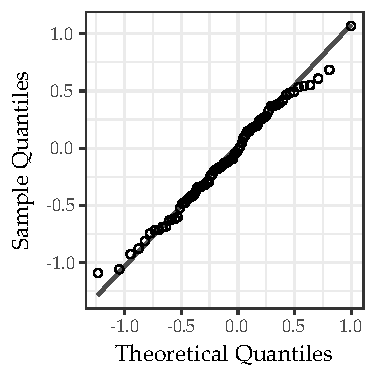
\includegraphics[width=0.32\textwidth]{./images/qq-norm-example}
			\label{fig:qq-example-a}%
			}%
		\subfloat[Heteroscedastic model]{%
			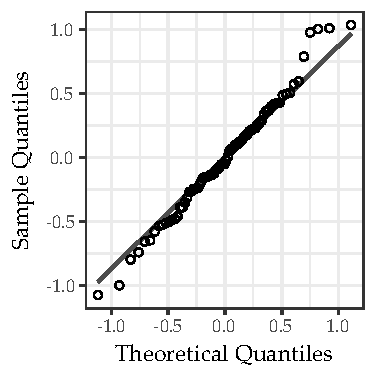
\includegraphics[width=0.32\textwidth]{./images/qq-hetero-example}
			\label{fig:qq-example-b}%
			}%
		\subfloat[Skewed model]{%
			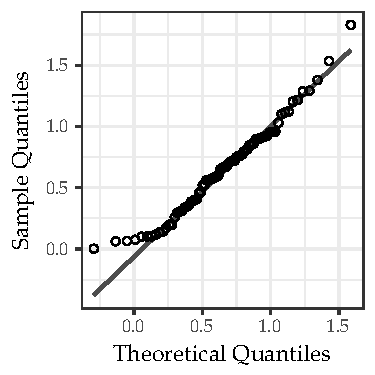
\includegraphics[width=0.32\textwidth]{./images/qq-skewed-example}
			\label{fig:qq-example-c}%
			}%
		\caption{Normal Q-Q plots for the three models simulated in \Cref{fig:models-example}}
		\label{fig:qq-example}
	\end{figure}

	Let us see if a residual plot can provide additional insight to the underlying models depicted in \Cref{fig:models-example} that could not be observed in the Q-Q plots in \Cref{fig:qq-example}.
	\begin{figure}[H]
		\centering
		\subfloat[Homoscedastic model]{%
			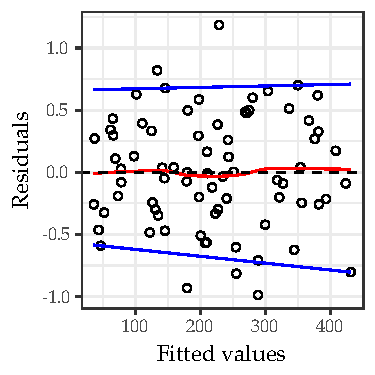
\includegraphics[width=0.32\textwidth]{./images/resid-norm-example}
			\label{fig:resid-example-a}%
			}%
		\subfloat[Heteroscedastic model]{%
			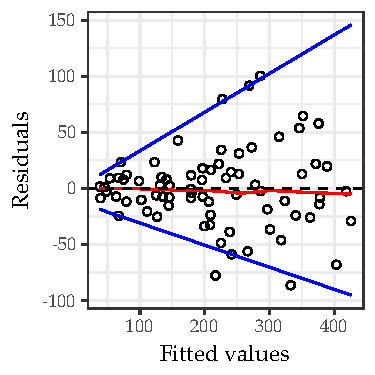
\includegraphics[width=0.32\textwidth]{./images/resid-hetero-example}
			\label{fig:resid-example-b}%
			}%
		\subfloat[Skewed model]{%
			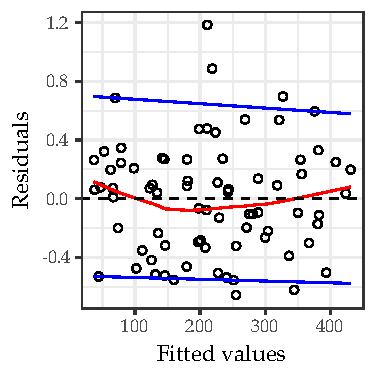
\includegraphics[width=0.32\textwidth]{./images/resid-skewed-example}
			\label{fig:resid-example-c}%
			}%
		\caption[Residual plots for the three models simulated in \Cref{fig:models-example}]{Residual plots for the three models simulated in \Cref{fig:models-example}, the red line is a smooth fit to the residuals, and the blue lines are the outer quantiles of the residuals}
		\label{fig:resid-example}
	\end{figure}

	In \Cref{fig:resid-example-a} and \Cref{fig:resid-example-c} we can see that the residuals appear to be roughly randomly distributed. However, for \Cref{fig:resid-example-c}, it is clear that the residuals are skewed, as the point pattern is densest somewhere other than the centre line; this tells us that the residuals do not follow a normal distribution at all. But we already knew this from \Cref{fig:qq-example-c}.

	In \Cref{fig:resid-example-b} we can see quite an extreme case of heteroscedasticity, as the magnitude of the residuals tends to increase with the fitted values, giving place to a prominent funnel shape. This tells us that there is some kind of correlation between the residuals and the predictors: $\epsilon_{i} \sim \hat{y}_{i} = f(x_{i})$.
	% \begin{figure}[H]
	% 	\centering
	% 	\subfloat[Homoscedastic model]{%
	% 		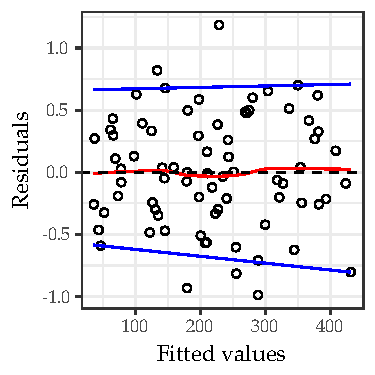
\includegraphics[width=0.32\textwidth]{./images/resid-norm-example}
	% 		\label{fig:resid-example-a}%
	% 		}%
	% 	\subfloat[Heteroscedastic model]{%
	% 		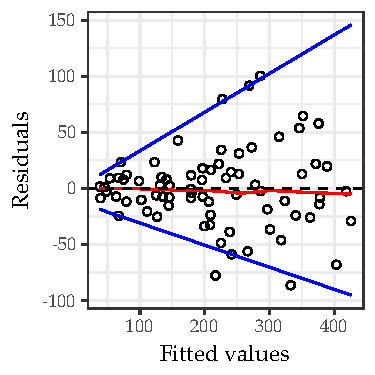
\includegraphics[width=0.32\textwidth]{./images/resid-hetero-example}
	% 		\label{fig:resid-example-b}%
	% 		}%
	% 	\subfloat[Skewed model]{%
	% 		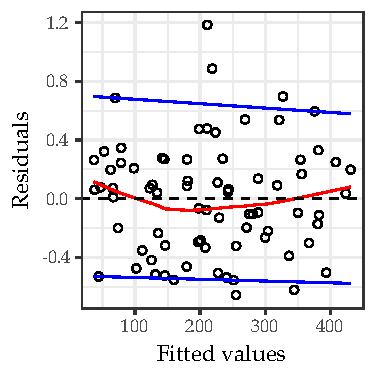
\includegraphics[width=0.32\textwidth]{./images/resid-skewed-example}
	% 		\label{fig:resid-example-c}%
	% 		}%
	% 	\caption{Residual plots for the three models simulated in \Cref{fig:models-example}, the red line is a smooth fit to the residuals, and the blue lines are the outer quantiles of the residuals}
	% 	\label{fig:resid-example}
	% \end{figure}

	As a last step, let us explore the results of performing the Lilliefors, correlation, and Breusch--Pagan tests in \Cref{tab:stat-tests-example}.
	\begin{table}[H]
		\centering
		\begin{tabular}{lccc}
			\toprule
			\toprule
			Model           & Lilliefors  & Correlation & Breusch--Pagan \\
			\midrule
			(a) Homoscedastic   & \num{0.649} & \num{1.000} & \num{0.312} \\
			(b) Heteroscedastic & \num{0.054} & \num{1.000} & \num{0.004} \\
			(c) Skewed          & \num{0.723} & \num{1.000} & \num{0.830} \\
			\bottomrule
		\end{tabular}
		\caption{List of $p$-values associated with the statistical hypothesis tests to respectively analyse normality, independence, and homoscedasticity of the residuals on the three simulated models}
		\label{tab:stat-tests-example}
	\end{table}

	From the results in \Cref{tab:stat-tests-example} we can see that the Lilliefors fails to reject the non-normality of the heteroscedastic and skewed models, when in fact only the homoscedastic model is simulated following a normal distribution, and that there is no correlation between the residuals and the fitted values for any of the models. More importantly, though, the Breusch--Pagan test successfully rejects homoscedasticity in the grossly heteroscedastic model.
\end{example}

%-----------------------------------------------------------------
\bigskip
To sum up, for linear regression with normal random errors having constant variance, the OLS theory of regression estimation provides clean, exact methods for analysis. But for generalisations to non-normal errors and non-constant variance, exact methods rarely exist, and we are faced with approximate methods based on linear approximations to estimators and central limit theorems. In the next section we will explore how resampling methods have the potential to provide a more accurate analysis.

\newpage
%-----------------------------------------------------------------
%	BACKGROUND: RESAMPLING THEORY
%	!TEX root = ./../main.tex
%-----------------------------------------------------------------
\subsection{Resampling methods}\label{sec:resampling}
Resampling methods are an indispensable tool in modern statistics. They involve repeatedly drawing samples from a data set and refitting a model of interest on each sample in order to obtain additional information about the fitted model. The term \emph{resampling} is used for any variety of methods for doing one of the following:
\begin{itemize}
	\item Estimating the precision of sample statistics (medians, variances, percentiles) by using subsets of available data (jackknifing) or drawing randomly with replacement from a set of data points (bootstrapping).
	\item Exchanging labels on data points when performing significance tests (permutation tests, also called exact tests, randomisation tests, or re-randomisation tests).
	\item Validating models by using random subsets (bootstrapping, cross validation).
\end{itemize}

Resampling approaches can be computationally expensive, because they involve fitting the same statistical method multiple times using different subsets of the studied data set. However, due to recent advances in computing power, the computational requirements of resampling methods generally are not prohibitive.

%-----------------------------------------------------------------
\subsubsection{The bootstrap in linear regression}\label{ssec:boot-theory}
The bootstrap is a method to derive properties (standard errors, confidence intervals and critical values) of the sampling distribution of estimators.

In the case of linear regression, when the assumptions on the residual error do not hold, there two quite different resampling methods: (a) resampling of the errors, and (b) resampling of the cases; being the second one more robust to failure of the model assumptions~\cite{Hinkley1997}.

For resampling the cases (or observations), one assumes the data is the sample from some bivariate distribution $f(X, Y)$. This will sometimes, but not often, mimic reality. Model \eqref{eq:lm-model} still applies, but with no assumption on the random errors $\epsilon_{i}$ other than independence.

With $f$ being the bivariate distribution of $(X, Y)$, it is appropriate to take $f$ to be the empirical distribution function (EDF) of the data pairs, and resampling will be from this EDF. The resampling simulation therefore involves sampling pairs with replacement from $(x_{i} , y_{i}), \dots , (x_{n} , y_{n})$. This is equivalent to taking
\begin{align}
	(x^{\ast}_{i} , y^{\ast}_{i}) = (x_{I} , y_{I}),
\end{align}
where $I$ is uniformly distributed on $\qty{1, 2, \dots, n}$. Then, simulated values $\hat{\beta}_{0}^{\ast}$, $\hat{\beta}_{1}^{\ast}$ the coefficient estimates are computed from $(x_{i}^{\ast} , y_{i}^{\ast}), \dots , (x_{n}^{\ast} , y_{n}^{\ast})$ using the OLS method which was applied to obtain the original estimates. This resampling algorithm can be summarised in \Cref{alg:bootstrap-theory}.

\IncMargin{1em}
\begin{algorithm}[H]
	\caption{Resampling the cases using bootstrap}
	\label{alg:bootstrap-theory}
	\DontPrintSemicolon
	\For{$r \gets 1$ \textbf{to} $R$}{
		$\text{(i)}$ Sample $i^{\ast}_{1}, \dots, i^{\ast}_{n}$ randomly with replacement from $\qty{1, 2, \dots, n}$.\;
		\For{$j \gets 1$ \textbf{to} $n$}{
			$\text{(ii)}$ Set $x_{j}^{\ast} = x_{i^{\ast}_{j}}$, $y_{j}^{\ast} = y_{i^{\ast}_{j}}$ \;
		}
		$\text{(iii)}$ Fit OLS regression to $(x_{i}^{\ast} , y_{i}^{\ast}), \dots , (x_{n}^{\ast} , y_{n}^{\ast})$.\;
		$\text{(iv)}$ Calculate estimates of $\hat{\beta}_{0,r}^{\ast}$ and $\hat{\beta}_{1,r}^{\ast}$.
	}
\end{algorithm}
\DecMargin{1em}

A great advantage of bootstrap is its simplicity. It is a straightforward way to derive estimates of standard errors and confidence intervals for complex estimators of complex parameters of the distribution, such as percentile points, proportions, and correlation coefficients. %Bootstrap is also an appropriate way to control and check the stability of the results.
Although for most problems it is impossible to know the true confidence interval, bootstrap is asymptotically more accurate than the standard intervals obtained using sample variance and assumptions of normality~\cite{Efron1993}.

%-----------------------------------------------------------------
\subsubsection{Permutation tests for comparing two populations}\label{ssec:perm-test-theory}
\nocite{Good2005}
\emph{Permutation tests} or randomisation tests are widely used in nonparametric statistics where a parametric form of the underlying distribution is not specified (or known).

Permutation tests for comparing two populations can be widely used in practice because of flexibility of the test statistic and minimal assumptions~\cite{Butar2008}. Consider sample of $m$ observations from population $A$ and $n$ observations from population $B$. Assume that under the null hypothesis $H_{0}$ there is no difference between a certain property of both populations; this could be the mean, the median, etc. Then any permutation of the observations between the two populations has the same chance to occur as any other permutation.

One could also perform parametric tests to test $H_{0}$, but they require the assumptions about the distribution of the characteristic in the population to be fulfilled. Permutation tests do not need fulfil the assumption about conformity with normal distribution and are as robust as parametric tests~\cite{Polko-Zajac2016}.

The essence of permutation tests is to determine a test statistic and then to evaluate the sample distribution of this statistic for all permutations of the populations. When calculations affect large number of permutations, a Monte Carlo method is applied (i.e., the permutations are random).

The steps for performing this kind of permutation test can be summarised in \Cref{alg:perm-test-theory}.

\newpage
\IncMargin{1em}
\begin{algorithm}[H]
	\caption{Permutation test for comparing two populations}
	\label{alg:perm-test-theory}
	\DontPrintSemicolon
	$\text{(i)}$ Define the null hypothesis, $H_{0}$, and the alternative.\;
	$\text{(ii)}$ Consider a test statistic that compares the populations which is large (small) if the null hypothesis is not true, and small (large) if it is true.\;
	$\text{(iii)}$ Calculate the true statistic of the data, $T$.\;
	\For{$r \gets 1$ \textbf{to} $R$}{
		$\text{(iv)}$ Create a new data set consisting of the data, randomly rearranged. Exactly how it is rearranged depends on the null hypothesis.\;
		$\text{(v)}$ Calculate the statistic for this new data set, $T^{\ast}$.\;
		$\text{(vi)}$ Compare the statistic $T^{\ast}$ to the true value, $T$.\;
	}
	$\text{(vii)}$ If the true statistic is greater (lower) than 95\% of the random values, then one can reject the null hypothesis at $p<0.05$.\;
\end{algorithm}
\DecMargin{1em}

A great advantage of the permutation tests exist for any test statistic, regardless of whether or not its distribution is known. Thus one is always free to choose the statistic which best discriminates between hypothesis and alternative and which minimises losses.


%-----------------------------------------------------------------
\section{Data}\label{sec:data-analysis}
%-----------------------------------------------------------------
%	DATA BACKGROUND
%	!TEX root = ./../main.tex
%-----------------------------------------------------------------
\subsection{Hurricane tracks}\label{ssec:hurdat}
\subsubsection{Description of the database}\label{ssec:hurdat-intro}
Although \citeauthor{Corral2010} analyse several ocean basins, we focus only on the North Atlantic (N.~Atl.) and the Northeast Pacific (E.~Pac.) Oceans. The reason to do this is the abundance of research on these two basins and the precision of the database provided by the National Hurricane Center (NHC)~\cite{o:NHC}: the HURDAT~\cite{o:hurdat2}.

Since both basins directly concern USA territories (especially the N.~Atl.), the government's efforts on improving the tracking and prediction technologies, routine satellite imagery has been used since as early as the late 1960s.

A major change between our data sets and the ones used by \textcite{Corral2010} is that the second-generation hurricane database (HURDAT2), has been developed this decade~\cite{Landsea2013}. The improvements of the revised version are mainly:
\begin{enumerate}[(i)]
	\item Inclusion of non-developing tropical depressions.
	\item Inclusion of systems that were added to the database after the end of each season.
\end{enumerate}
Also, the ongoing post-storm analysis reviews of the tropical-cyclones have revised several storms~\cite{o:hurdat-comparison}, particularly important in the 1851--1960 era.

\medskip
Recently, in June 2018, \textcite{Delgado2018} have revised and updated the HURDAT2 data set. This revision includes storms from 2017, as well as a revision of the 1954--63 era for the North Atlantic data. Nonetheless, the analysis is done using the 2016 data sets, as it would require a lot of effort to clean the new data and make sure no major change has been done introduced into historical data.

These raw data sets used can be downloaded from \url{http://www.aoml.noaa.gov/hrd/hurdat/hurdat2-1851-2016-apr2017.txt} (N.~Atl.) and \url{http://www.aoml.noaa.gov/hrd/hurdat/hurdat2-nepac-1949-2016-apr2017.txt} (E.~Pac.).

%-----------------------------------------------------------------
\subsubsection{Data structure}
The format of the HURDAT2 data sets is documented at~\cite{Landsea2014,Landsea2016}. A record of data is recorded once every 6 hours for each storm (although there are additional records for certain storms, specially those marking the landfall of a storm). The record is comprised of the date and time, storm identifier, system status (cf. tropical-cyclone category), latitude and longitude of the centre of the storm, the sustained surface wind speed (in knots) observed in the storm, and several other properties that are not relevant in this study.

In \Cref{hd:hurdat-head} one can see the structure of the cleaned data illustrate the variables we use in the study directly available in the raw data sets, as well as the format (data type\footnote{In computer science and computer programming, a data type or simply type is a classification of data which tells the compiler or interpreter how the programmer intends to use the data. }) of the observational record data.
\begin{table}[H]
	\centering
	\ttfamily
	\resizebox{\textwidth}{!}{%
	\begin{tabular}{r r r r  r r r r r}
		\toprule
		\toprule
		storm.id & storm.name & n.obs &           date.time &         status &   lat &  long &  wind & storm.year \\
		   <chr> &      <chr> & <int> &              <dttm> &         <fctr> & <dbl> & <dbl> & <dbl> &      <dbl> \\
		\midrule
		AL011851 &    UNNAMED &    13 & 1851-06-25 00:00:00 &      Hurricane &  28.0 & -94.8 &    80 &       1851 \\
		AL011851 &    UNNAMED &    13 & 1851-06-25 06:00:00 &      Hurricane &  28.0 & -95.4 &    80 &       1851 \\
		AL011851 &    UNNAMED &    13 & 1851-06-25 12:00:00 &      Hurricane &  28.0 & -96.0 &    80 &       1851 \\
		AL011851 &    UNNAMED &    13 & 1851-06-25 18:00:00 &      Hurricane &  28.1 & -96.5 &    80 &       1851 \\
		AL011851 &    UNNAMED &    13 & 1851-06-26 00:00:00 &      Hurricane &  28.2 & -97.0 &    70 &       1851 \\
		AL011851 &    UNNAMED &    13 & 1851-06-26 06:00:00 & Tropical storm &  28.3 & -97.6 &    60 &       1851 \\
		\bottomrule
	\end{tabular}}
	\caption{Excerpt of the North Atlantic data set}
	\label{hd:hurdat-head}
\end{table}

A map displaying the studied hurricane tracks for the North Atlantic and Northeast Pacific basins can be seen in \Cref{fig:full-map}.

%-----------------------------------------------------------------
%	DATA BACKGROUND
%	!TEX root = ./../main.tex
%-----------------------------------------------------------------
\subsection{Sea surface temperature}\label{ssec:sst}

\subsubsection{Description of the database}\label{ssec:hadisst-intro}
There are several sea surface temperature (SST) databases, with different time-steps (e.g., daily, weekly, monthly, and so on), domains (i.e., global or specific regions), and data resolutions; each used for different analyses of climatological nature~\cite{o:sst-comparison, Rayner2003}.

The Met Office~\cite{o:met-office} Hadley Centre's sea ice and sea surface temperature database, HadISST1~\cite{o:hadisst1}, is a unique combination of monthly globally complete fields of SST and sea ice concentration on a latitude-longitude grid from 1871. In \Cref{fig:sst-raster-map} we can see a sample from the data set to illustrate the grid structure.

Although there is a revised HadISST.2 database~\cite{o:hadisst2}, we use the HadISST1 database, as it is the one used in \citeauthor{Corral2010}'s, \citeauthor{Webster2005}'s and several other authors's climate analyses.

The main reason to do so, however, is that HadISST.2 contains more ocean grid boxes and introduces a different method to calculate the monthly temperatures, making it quite incompatible with HadISST1 (as opposed to the revised HURDAT2 database, which is just an improved version of the old database, without introducing changes in the methodology of analysis or in the structure of the data).

\begin{figure}[H]
	\centering
	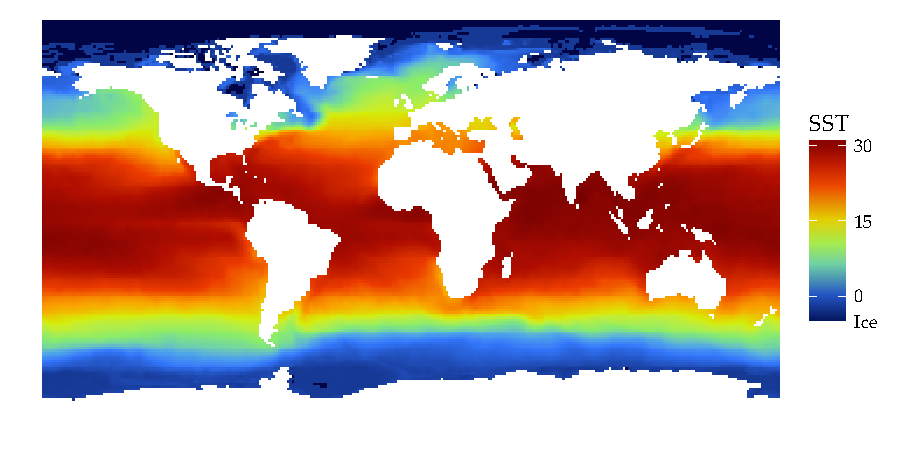
\includegraphics[width=\textwidth]{images/sst-raster-map}
	\caption{Global SST (in \si{\celsius}) map from December 2015}
	\label{fig:sst-raster-map}
\end{figure}

%-----------------------------------------------------------------
\subsubsection{Data structure}
The format of the HadISST1 database is documented at~\cite{o:hadisst1-format}. The data are available in netCDF format, which is constructed using raster data.

A raster brick consists of a matrix of cells (or pixels) organised into a grid where each cell contains a value representing information, such as temperature in our case. Each matrix can also be comprised of layers (as illustrated in \Cref{fig:raster}); in the HadISST1 database, each matrix layer represents a different month.
\begin{figure}[H]
	\centering
	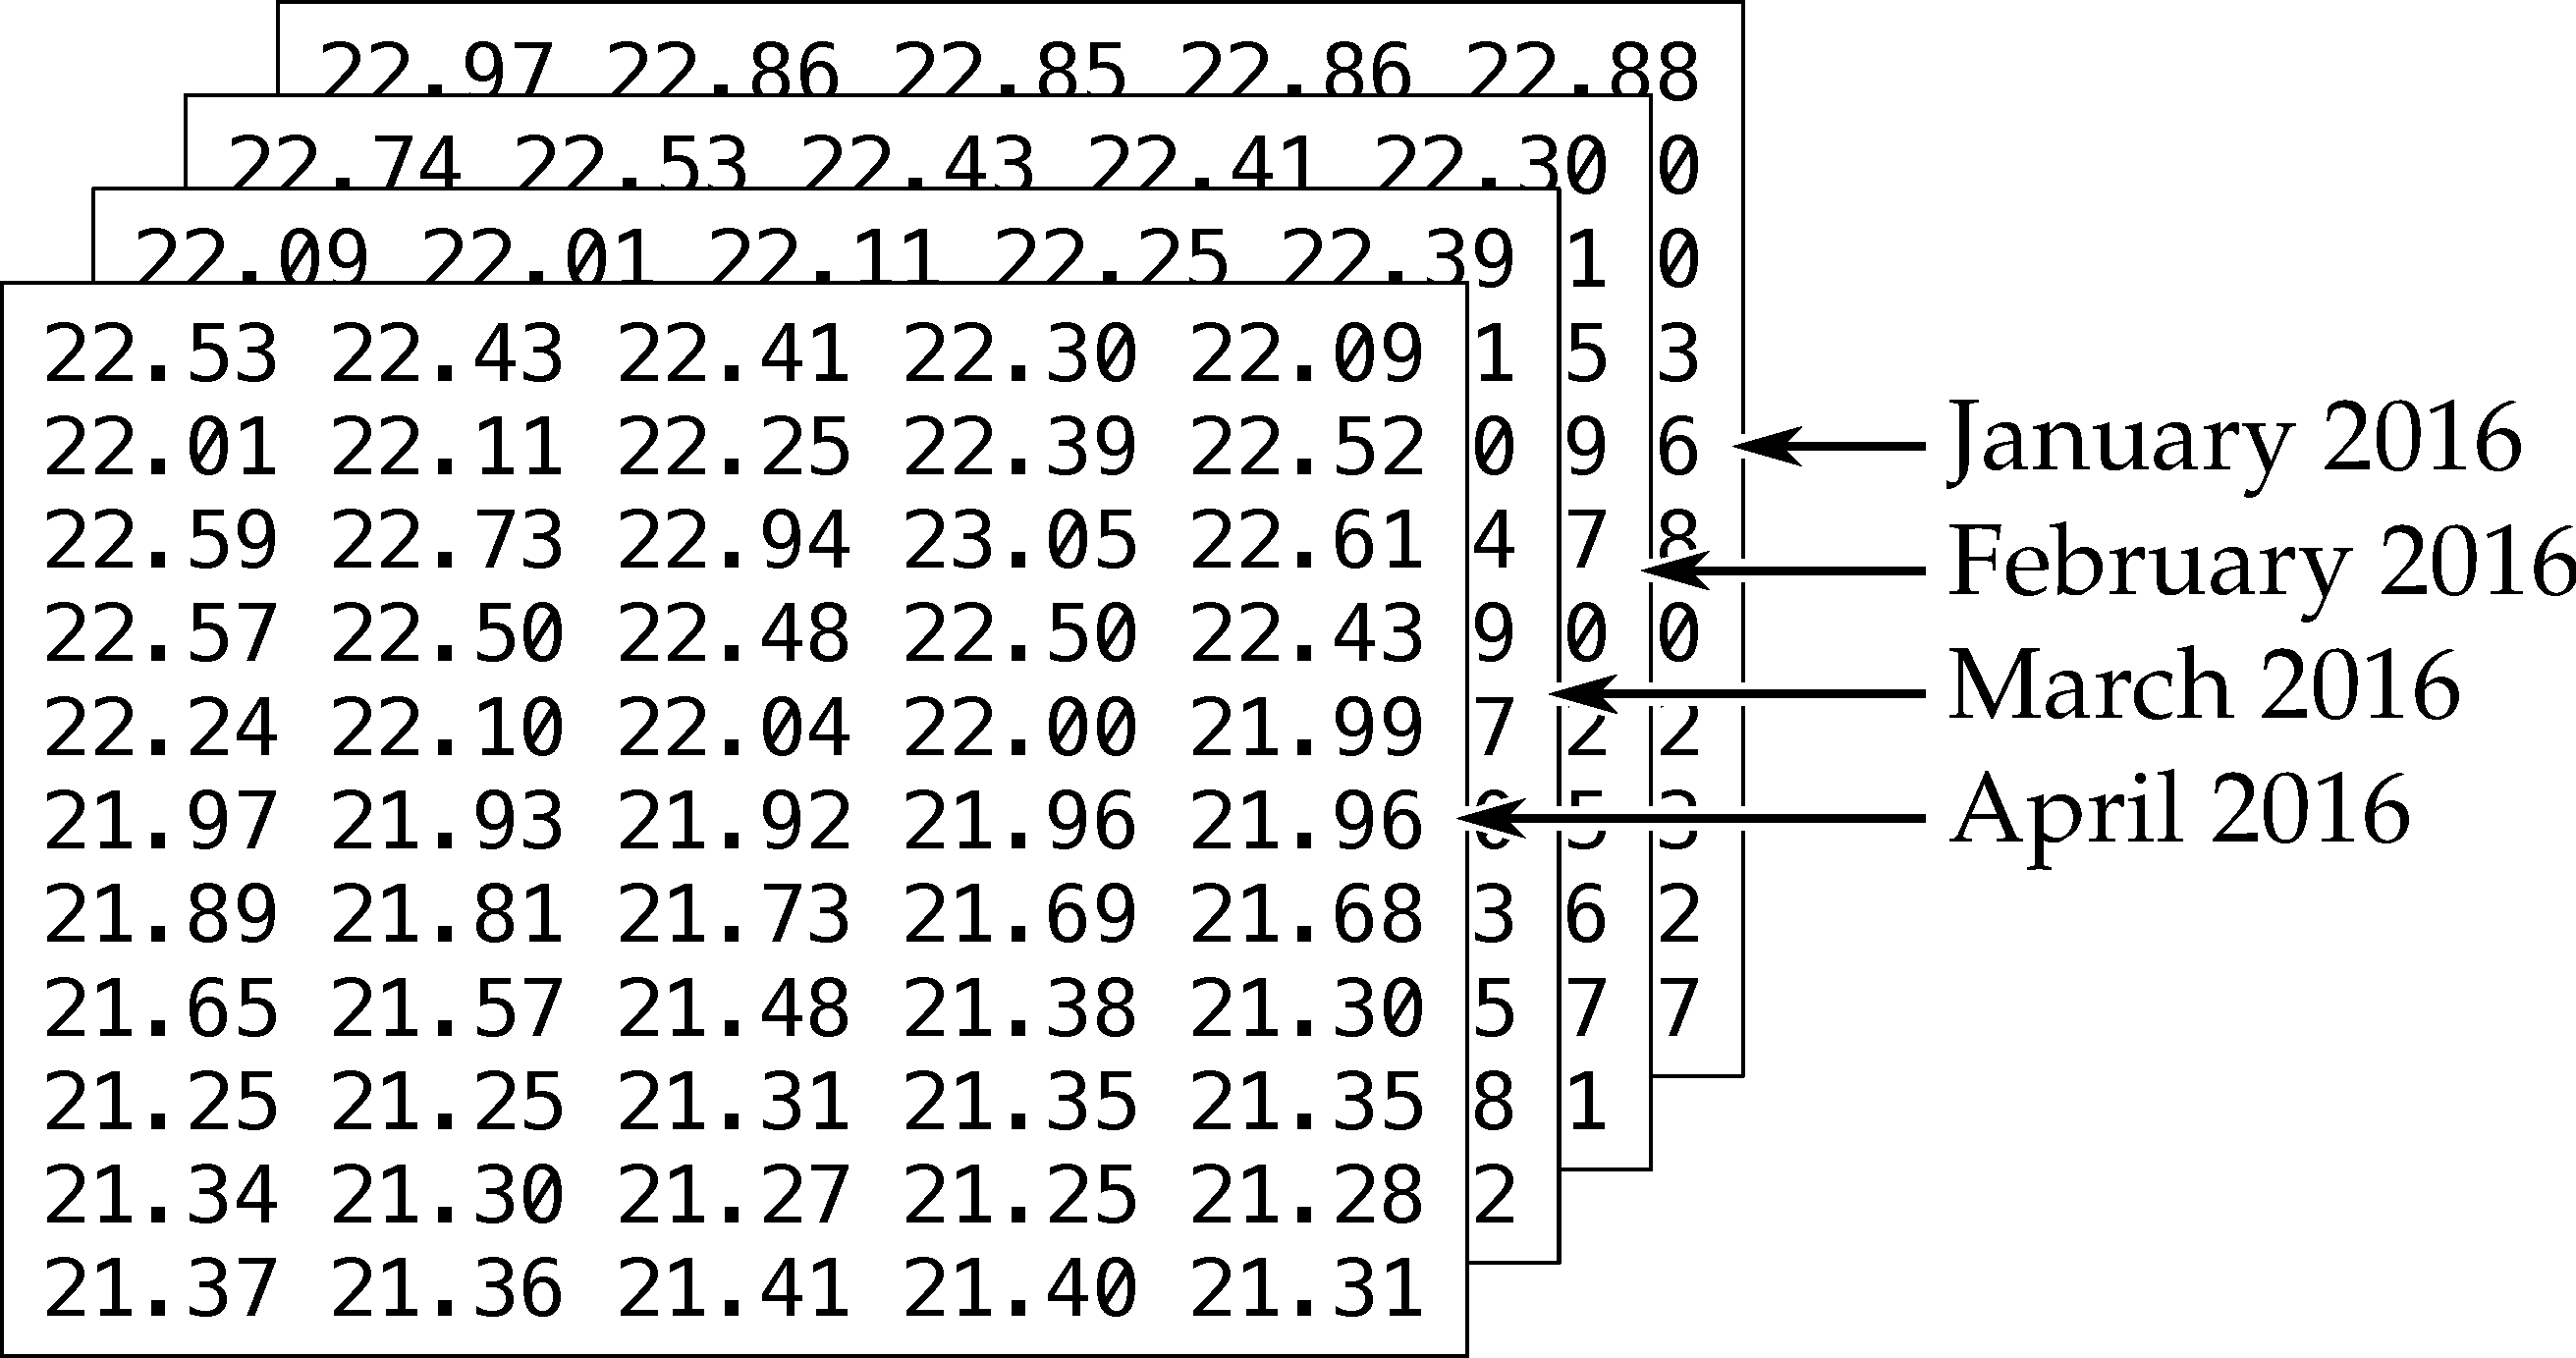
\includegraphics[width=0.7\textwidth]{images/raster}
	\caption{Simple diagram of the internal structure of a raster brick}
	\label{fig:raster}
\end{figure}

The data set used can be downloaded from \url{http://www.metoffice.gov.uk/hadobs/hadisst/data/HadISST_sst.nc.gz}.

\bigskip
% \todo[inline]{paragraph about the SST class}
In \Cref{hd:sst-head} one can see the structure of the result from the SST classification of the years into low-SST and high-SST to illustrate the variables we use, as well as the data type of the SST data. Note that the classification is unique to each of the basins.
\begin{table}[H]
	\centering
	\ttfamily
	\begin{tabular}{r r r r}
		\toprule
		\toprule
		year & sst & sst.norm & sst.class \\
		<date> &   <dbl>   &  <dbl> &    <chr> \\
		\midrule
		1966-01-01 & 27.47 & 0.9979934 &  low \\
		1967-01-01 & 27.19 & 0.9879054 &  low \\
		1968-01-01 & 27.34 & 0.9933687 &  low \\
		1969-01-01 & 27.75 & 1.0083072 & high \\
		1970-01-01 & 27.36 & 0.9940200 &  low \\
		1971-01-01 & 27.04 & 0.9825272 &  low \\
		\bottomrule
	\end{tabular}
	\caption{Excerpt of the results from the SST analysis for the North Atlantic basin}
	\label{hd:sst-head}
\end{table}

%-----------------------------------------------------------------
%	DATA BACKGROUND
%	!TEX root = ./../main.tex
%-----------------------------------------------------------------
\subsection{Activity windows}\label{ssec:act-windows}
Even though recent improvements have been made to the HURDAT2 database, \cite{o:hurdat-comparison,Landsea2014,Landsea2016}, following the methodology of \citeauthor{Corral2010}, we intentionally limit this study to the satellite era.

In \cite{Webster2005}, \citeauthor{Webster2005} go into more details about the activity windows for the hurricane tracks data as well as the sea surface temperature used by researchers in the past. In \Cref{tab:act-windows} we can see a summary of the spatial and temporal activity windows we use for each basin based on the information available in the previously mentioned papers; we also include the amount of analysed tropical-cyclones $N$, the amount of occurrences in low-SST years $N_{\text{low}}$, the amount of occurrences in high-SST years $N_{\text{high}}$, as well as the size of the entire data set $N_{tot}$.
\begin{table}[H]
	\centering
	\resizebox{\textwidth}{!}{%
	\begin{tabular}{l c c c c c c c c}
		\toprule
		\toprule
		Basin & Years & Season & Longitude & Latitude & $N$ & $N_{\text{low}}$ & $N_{\text{high}}$ & $N_{tot}$ \\
		\midrule
		N.~Atl. & 1966--2016 & June--October & \ang{90}W--\ang{20}W  & \ang{5}N--\ang{25}N & \num{771} & \num{365} & \num{406} & \num{1756}  \\
		E.~Pac. & 1986--2016 & June--October & \ang{120}W--\ang{90}W & \ang{5}N--\ang{20}N & \num{594} & \num{238} & \num{356} & \num{1071}  \\
		\bottomrule
	\end{tabular}}
	\caption{Spatial and temporal activity windows for each basin}
	\label{tab:act-windows}
\end{table}

In \Cref{fig:full-map} we can see a map showing all the storms analysed for both basins (N.~Atl. and E.~Pac.), already divided by SST class, and the spatial window for the $\ev{\text{SST}}$ calculation highlighted in green.
\begin{figure}[H]
	\centering
	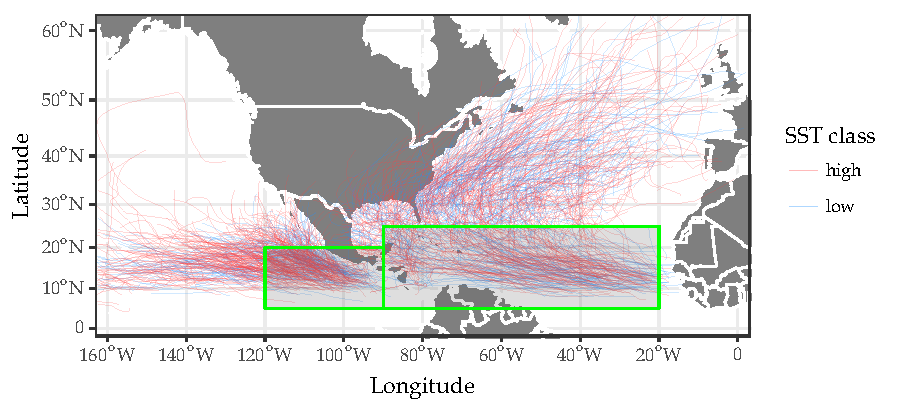
\includegraphics[width=\textwidth]{images/full-map}
	\caption{Tropical-cyclones best tracks for the North Atlantic and Northeast Pacific Oceans}
	\label{fig:full-map}
\end{figure}

%-----------------------------------------------------------------
\subsection{Unified data set}\label{ssec:unified-data-set}
For this study, we have developed a unified data set that summarises the relevant variables of each analysed tropical-cyclone using data from the HURDAT2 and the HadISST1.

In \Cref{hd:unified-dataset-head} one can see the structure of the unified data set to illustrate the variables we use, as well as their data type.
\begin{table}[H]
	\centering
	\ttfamily
	\resizebox{\textwidth}{!}{%
	\begin{tabular}{r r r r r r r r r r r r r}
		\toprule
		\toprule
		storm.id & storm.name & n.obs & storm.duration &    storm.pdi & max.wind & mean.wind & mean.sq.wind & storm.year & basin &   sst & sst.norm & sst.class \\
		<chr>    & <chr>      & <int> &          <dbl> &        <dbl> &    <int> &     <dbl> &        <dbl> &      <int> & <chr> & <dbl> &    <dbl> &     <chr> \\
		\midrule
		AL011966 & ALMA       &    42 &            252 &  34632626747 &      110 &      56.4 &        3750  &       1966 & NATL  &  27.6 &    0.998 &       low \\
		AL021966 & BECKY      &     9 &             54 &   3413930334 &       65 &      46.1 &        2353. &       1966 & NATL  &  27.6 &    0.998 &       low \\
		AL031966 & CELIA      &    36 &            216 &   7839872104 &       70 &      35.4 &        1488. &       1966 & NATL  &  27.6 &    0.998 &       low \\
		AL041966 & DOROTHY    &    37 &            222 &  21340832518 &       75 &      54.9 &        3211. &       1966 & NATL  &  27.6 &    0.998 &       low \\
		AL051966 & ELLA       &    26 &            156 &   4646503652 &       45 &      37.7 &        1487. &       1966 & NATL  &  27.6 &    0.998 &       low \\
		AL061966 & FAITH      &    69 &            414 & 120569417711 &      110 &      79.0 &        6722. &       1966 & NATL  &  27.6 &    0.998 &       low \\
		\bottomrule
	\end{tabular}}
	\caption{Excerpt of the North Atlantic data set}
	\label{hd:unified-dataset-head}
\end{table}

This unified data sets for the North Atlantic and Northeast Pacific basins can be downloaded from the GitLab repository of this project~\cite{o:gitlab-repo} in \texttt{CSV} format.

Alternatively, these data sets have been packaged into an R package called \texttt{HurdatHadISSTData} \cite{o:gitlab-data-repo}, and can be installed using the \texttt{devtools} package:
\begin{lstlisting}
library(devtools)
install_git("https://gitlab.com/aldomann/hurdat-hadisst-data.git")
\end{lstlisting}

The names of these data sets in the \texttt{HurdatHadISSTData} package are:
\begin{itemize}
	\item \texttt{tc.pdi.natl} -- Data set for the North Atlantic basin.
	\item \texttt{tc.pdi.epac} -- Data set for the Northeast Pacific basin.
	\item \texttt{tc.pdi.all} -- Data set for both basins.
\end{itemize}

%-----------------------------------------------------------------
%	DATA: ON DEVELOPING SYSTEMS
%	!TEX root = ./../main.tex
%-----------------------------------------------------------------
% \newpage
\subsection{On non-developing systems}
% As we mentioned in~\cref{sec:pdi-vs-sst}, we want to find a correlation between the $PDI$ and the duration of the storms, or their wind speeds. Instead of using the whole tropical-cyclones data set as is, we will separate developing from non-developing systems.
Tropical-cyclones that surpass the $\SI{33}{\knot}$ wind speed threshold are called \emph{developing systems}, while the ones that do not do so are called \emph{non-developing systems}. In terms of hydrodynamics, the major difference between developing and non-developing systems is that the developing have a distinct area of low height or low pressure centred on the system, i.e., they form cyclones~\cite{McBride1979}.

This means that even though all tropical-cyclones behave thermodynamically in the same way throughout their lifetime (the $PDI$ calculation is valid for all their life span), the wind speeds evolve rather differently depending on the development status of the storm.

% For this reason, one should play on the cautious side and study developing and non-developing systems separately, as they represent different physical systems.

\medskip
% \todo[inline]{NON-STATIONARY}
Apart from this physical description, from a statistical point of view, one can see that non-developing systems constitute a \emph{nonstationary} time series for the North Atlantic data (\Cref{fig:natl-storms-ts} and \Cref{tab:natl-storms-ts-stationarity}); this means the distribution of the storms alters with alterations in time.

% \todo{Expand this paragraph}
\begin{figure}[H]
	\centering
	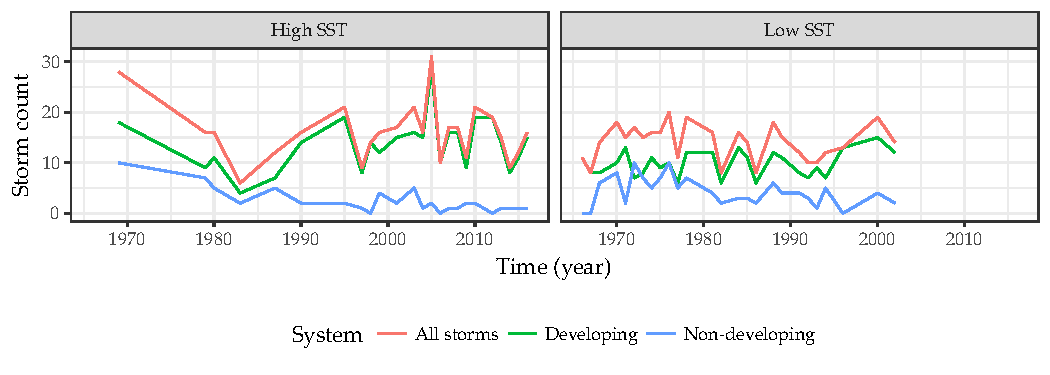
\includegraphics[width=\textwidth]{images/natl-storms-ts}
	\caption{Time series of storm occurrences for the North Atlantic basin, emphasising into non-developing systems and developing systems}
	\label{fig:natl-storms-ts}
\end{figure}

\begin{table}[H]
	\centering
	\begin{tabular}{lccc}
		\toprule
		\toprule
		Subset     & Non-developing & Developing & All storms \\
		\midrule
		All storms &  $0.0205$      & $\geq 0.1$ & $\geq 0.1$ \\
		Low SST    &  $0.0233$      & $\geq 0.1$ & $\geq 0.1$ \\
		High SST   &  $0.0429$      & $\geq 0.1$ & $\geq 0.1$ \\
		\bottomrule
		\bottomrule
	\end{tabular}
	\caption{List of $p$-values associated with the Kwiatkowski--Phillips--Schmidt--Shin test to analyse stationarity of the storm occurrences for the North Atlantic basin}
	\label{tab:natl-storms-ts-stationarity}
\end{table}

For the Northeast Pacific data (\Cref{fig:epac-storms-ts} and \Cref{tab:epac-storms-ts-stationarity}), stationarity is rejected only for the time series without separation of the storms by SST class.

\begin{figure}[H]
	\centering
	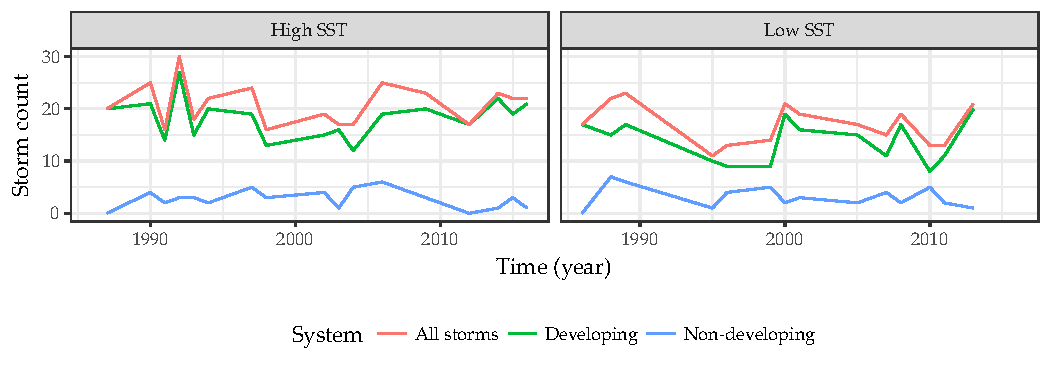
\includegraphics[width=\textwidth]{images/epac-storms-ts}
	\caption{Time series of storm occurrences for the Northeast Pacific basin, emphasising into non-developing systems and developing systems}
	\label{fig:epac-storms-ts}
\end{figure}

\begin{table}[H]
	\centering
	\begin{tabular}{lccc}
		\toprule
		\toprule
		Subset     & Non-developing & Developing & All storms \\
		\midrule
		All storms &  $0.0294$      & $\geq 0.1$ & $\geq 0.1$ \\
		Low SST    &  $0.0732$      & $\geq 0.1$ & $\geq 0.1$ \\
		High SST   &  $0.0733$      & $\geq 0.1$ & $\geq 0.1$ \\
		\bottomrule
		\bottomrule
	\end{tabular}
	\caption{List of $p$-values associated with the Kwiatkowski--Phillips--Schmidt--Shin test to analyse stationarity of the storm occurrences for the Northeast Pacific basin}
	\label{tab:epac-storms-ts-stationarity}
\end{table}

The issue with this is that when nonstationary time series are used in a regression model one may obtain apparently significant relationships from unrelated variables. This phenomenon is called \emph{spurious regression}~\cite{Phillips1986}. For example, if the series is consistently increasing over time, the sample mean and variance will grow with the size of the sample, and they will always underestimate the mean and variance in future periods. And if the mean and variance of a series are not well-defined, then neither are its correlations with other variables.

One should be cautious, therefore, about trying to extrapolate regression models fitted to nonstationary data.

\bigskip
Although we do not perform a direct regression analysis on the time series of storm occurrences, our data is temporally distributed following this time series. Thus, to be on the cautious side, as they represent different physical systems and may introduce problems in the regression analysis, for our study, we opt to exclude non-developing systems altogether.

One could argue that this is not necessary for the Northeast Pacific basin, but to be consistent in the methodology applied to both basins, we exclude non-developing systems as well.


%-----------------------------------------------------------------
\section{Regression analysis using resampling methods}\label{sec:regr-analysis-boot}
%-----------------------------------------------------------------
%	BOOTSTRAP: DISTRIBUTIONAL PROPERTIES OF THE DATA
%	!TEX root = ./../main.tex
%-----------------------------------------------------------------
\subsection{Distributional properties of the data}\label{sec:distribution-analysis}
It is important to notice that the relationships between a storm's $PDI$ and its lifetime are of non-linear nature. This naturally means that our regressions need to follow a so-called log--log model:
\begin{align}\label{eq:lm-model-bis}
	\log \Psi = \beta_{0} + \beta_{1} \log \Phi + \epsilon,
	\tag{\ref{eq:lm-model} bis}
\end{align}
where $\log \Psi \equiv Y$ and $\log \Phi \equiv X$.

We do not know exactly how the $PDI$ and the lifetime of the storms are exactly correlated; we just suspect there is a correlation. For this reason, we not only compute the $Y(X)$ fit for each data set, but also $X(Y) = \hat{\beta}_{0} + \hat{\beta}_{1} Y$, which is calculated as stated in \cref{sec:lm-coefs} just interchanging the role of $X$ and $Y$.

\medskip
Before performing the regression analysis we should study, however, the bivariate distribution of the data and the marginal distributions of the $PDI$ and the lifetime of storms to see any difference between the two populations that are result of the separation of the storms by SST class.

%-----------------------------------------------------------------
\subsubsection{Bivariate lognormal distribution}\label{sec:bvln-distribution}
\nocite{Thomopoulos2017}
The bivariate lognormal has two variables, $X_{1}$ and $X_{2}$, that are jointly related, and has five parameters, $\mu_{1}$, $\mu_{2}$, $\sigma_{1}^{2}$, $\sigma_{2}^{2}$, and $r$:
\begin{align}
	f(X_{1}, X_{2}) \sim \mc{BVLN}(\mu_{1}, \mu_{2}, \sigma_{1}^{2}, \sigma_{2}^{2}, r).
\end{align}

The marginal distributions are lognormally distributed, i.e., the logarithm of them is normally distributed:
\begin{align}
	\log X_{1} \sim \mc{N}(\mu_{1}, \sigma_{1}^{2})
	\qc
	\log X_{2} \sim \mc{N}(\mu_{2}, \sigma_{2}^{2})
	,
\end{align}
and when the value of one of the variables is known, the distribution on the other is also normally distributed. This, naturally implies that the joint distribution of the logarithm of the variables follows a bivariate normal distribution:
\begin{align}
	f(\log X_{1}, \log X_{2}) \sim \mc{BVN}(\mu_{1}, \mu_{2}, \sigma_{1}^{2}, \sigma_{2}^{2}, r) .
\end{align}

\Cref{fig:bvn-example} shows a bivariate normal distribution to illustrate both the joint distribution between the two variables $X_{1}$ and $X_{2}$ and their respective marginal distributions.
\begin{figure}[H]
	\centering
	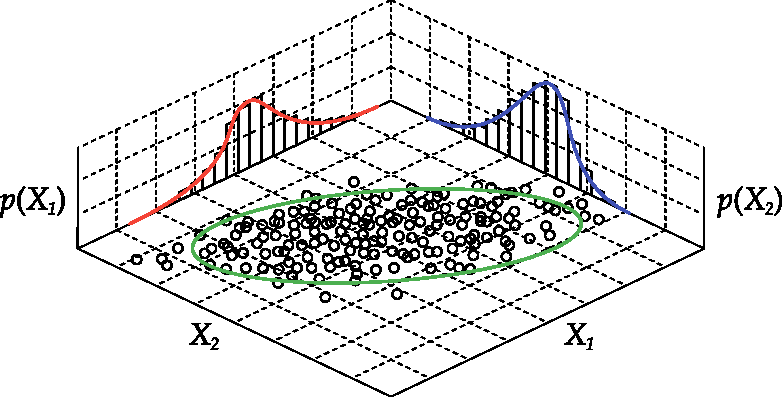
\includegraphics[width=0.75\textwidth]{images/bvn-example}
	\caption{Bivariate normal distribution $f(X_{1}, X_{2})$ and the marginal distributions of $X_{1}$ and $X_{2}$}
	\label{fig:bvn-example}
\end{figure}

% \medskip
In \Cref{fig:natl-bvln} and \Cref{fig:epac-bvln} we can see the bivariate lognormal distributions of the $PDI$ and lifetime of the storms for the North Atlantic and Northeast Pacific basins separating storms by SST class.

\begin{figure}[H]
	\centering
	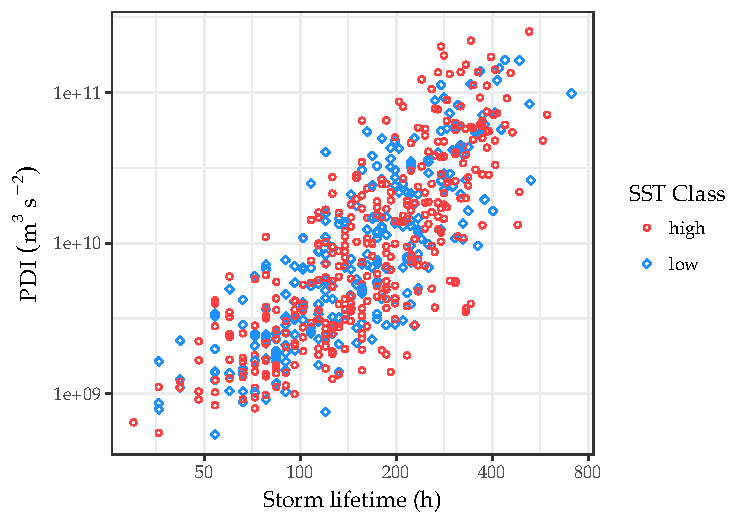
\includegraphics[width=0.8\textwidth]{images/natl-bvln}
	\caption{Bivariate lognormal distribution $f(PDI, \text{lifetime})$ of the hurricane observations for the North Atlantic basin}
	\label{fig:natl-bvln}
\end{figure}

\begin{figure}[H]
	\centering
	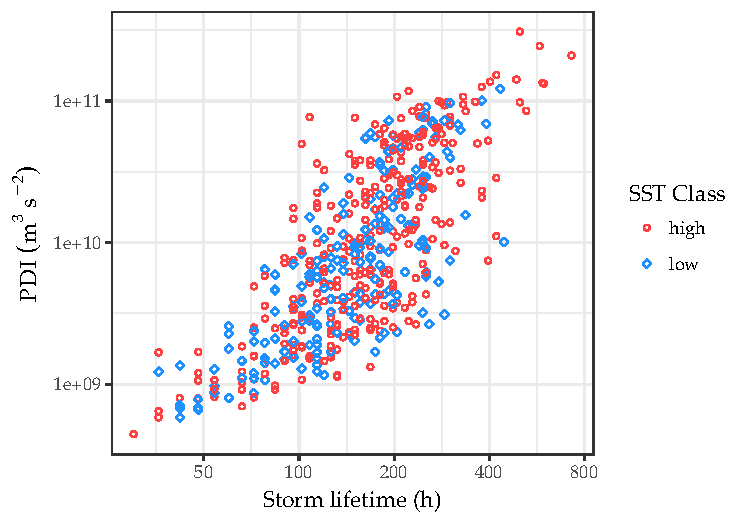
\includegraphics[width=0.8\textwidth]{images/epac-bvln}
	\caption{Bivariate lognormal distribution $f(PDI, \text{lifetime})$ of the hurricane observations for the Northeast Pacific basin}
	\label{fig:epac-bvln}
\end{figure}

The first thing to notice is that, as our hypothesis predicts, although the joint distributions seem to overlap, the expected value $(\mu_{PDI}, \mu_{\text{lifetime}})$ seems to be different for the distributions associated to each SST class. To see this more clearly, we should perform a descriptive univariate analysis of the marginal distributions.

%-----------------------------------------------------------------
% \newpage
\subsubsection{Descriptive univariate analysis of the marginals}\label{ssec:univariate}

% \todo[inline]{Show that we care about the expected values, not the distributions themselves. If possible, add $t$ test to compare them}

In \Cref{fig:natl-marginals-pdi} and \Cref{fig:natl-marginals-lifetime} we can see the marginal distributions of the $PDI$ and lifetime, in logarithmic scale, for the North Atlantic basin data, separating the data by SST class. For the marginal analysis we also show the expected value $\mu$ as a dashed line. Similarly, in \Cref{fig:epac-marginals-pdi} and \Cref{fig:epac-marginals-lifetime} we show the same marginal distributions for the Northeast Pacific basin data.

A statistical summary of the marginals for both basins can be seen in \Cref{tab:natl-marginals-stats} and \Cref{tab:epac-marginals-stats}.

\medskip
We can see that the marginals do not follow exactly a normal distribution for the $PDI$. This is expected, as \textcite{Corral2010} show that the $PDI$ distributions can be characterised by a power-law decay in their central regions. The lifetime marginal distributions do, as it is expected from a bivariate lognormal distribution, roughly follow a normal distribution.

The results show that the expected value $(\mu_{PDI}, \mu_{\text{lifetime}})$ of the joint distributions are displaced to the right-upper corner for high-SST years. This can be clearly seen in the fact that high-SST years have a longer right tail on account of having more available energy from the sea, and as a result displace the mean of the population $\mu$ to higher values as well. This is both reflected in the $PDI$ and the storm lifetime.

 % are not the same for storms occurred in low-SST years and high-SST years, but the expected values for the high-SST years are higher, supporting our hypothesis that high-SST years should have a longer right tail on account of having more available energy from the sea, displacing the expected value $(\mu_{PDI}, \mu_{\text{lifetime}})$ of the joint distribution to the upper-right corner.

\begin{figure}[H]
	\centering
	\subfloat[Marginal distribution of the $PDI$]{%
		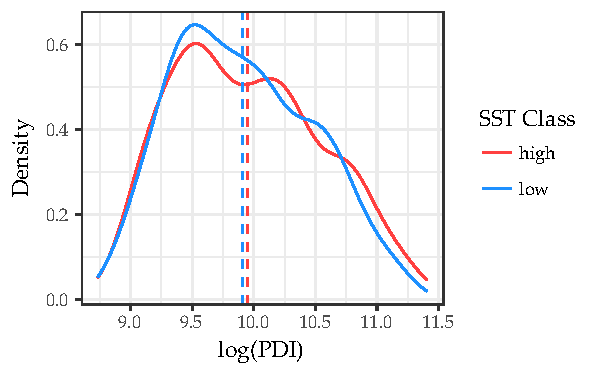
\includegraphics[width=0.5\textwidth]{./images/natl-marginals-pdi}
		\label{fig:natl-marginals-pdi}%
		}%
	\subfloat[Marginal distribution of the lifetime]{%
		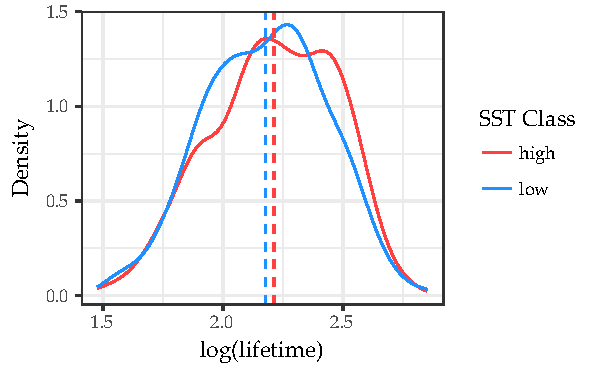
\includegraphics[width=0.5\textwidth]{./images/natl-marginals-lifetime}
		\label{fig:natl-marginals-lifetime}%
		}%
	\caption{Marginal analysis for the variables of the bivariate lognormal distribution for the North Atlantic basin data}
	\label{fig:natl-marginals}
\end{figure}

\vspace{-5pt}
\begin{table}[H]
	\centering
	\begin{tabular}{lccc}
		\toprule
		\toprule
		Marginal variable & Data & Mean $\mu$            & Median \\
		\midrule
		\multirow{2}{*}{$\log(PDI)$}
		 & Low-SST               & \num{9.91 \pm 0.04} & \num{9.86 \pm 0.04} \\
		 & High-SST              & \num{9.95 \pm 0.03} & \num{9.91 \pm 0.04} \\
		\midrule
		% \cmidrule(l){2-5}
		\multirow{2}{*}{$\log(\text{lifetime})$}
		 & Low-SST               & \num{2.18 \pm 0.02} & \num{2.19 \pm 0.02} \\
		 & High-SST              & \num{2.21 \pm 0.01} & \num{2.23 \pm 0.02} \\
		\bottomrule
	\end{tabular}
	\caption{Statistical summary for the low-SST and high-SST subsets of the marginals of the bivariate lognormal distribution for the North Atlantic basin data}
	\label{tab:natl-marginals-stats}
\end{table}

\vspace{-5pt}
\begin{figure}[H]
	\centering
	\subfloat[Marginal distribution of the $PDI$]{%
		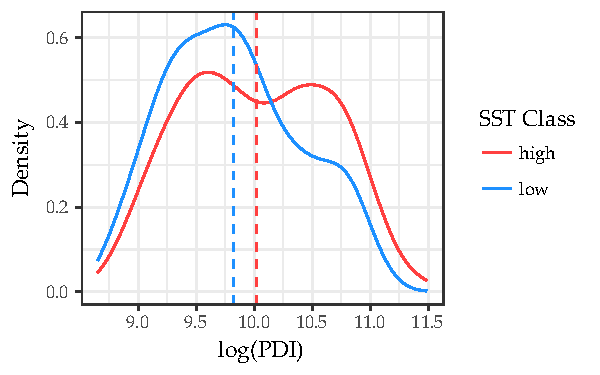
\includegraphics[width=0.5\textwidth]{./images/epac-marginals-pdi}
		\label{fig:epac-marginals-pdi}%
		}%
	\subfloat[Marginal distribution of the lifetime]{%
		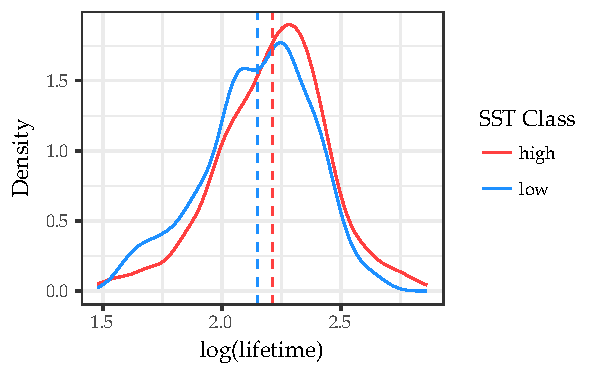
\includegraphics[width=0.5\textwidth]{./images/epac-marginals-lifetime}
		\label{fig:epac-marginals-lifetime}%
		}%
	\caption{Marginal analysis for the variables of the bivariate lognormal distribution for the Northeast Pacific basin data}
	\label{fig:epac-marginals}
\end{figure}


\begin{table}[H]
	\centering
	\begin{tabular}{clcc}
		\toprule
		\toprule
		Marginal variable & Data & Mean $\mu$            & Median \\
		\midrule
		\multirow{2}{*}{$\log(PDI)$}
		 & Low-SST               & \num{9.82 \pm 0.04} & \num{9.78 \pm 0.05} \\
		 & High-SST              & \num{10.0 \pm 0.04} & \num{9.99 \pm 0.04} \\
		\midrule
		% \cmidrule(l){2-5}
		\multirow{2}{*}{$\log(\text{lifetime})$}
		 & Low-SST               & \num{2.15 \pm 0.02} & \num{2.18 \pm 0.02} \\
		 & High-SST              & \num{2.21 \pm 0.01} & \num{2.23 \pm 0.02} \\
		\bottomrule
	\end{tabular}
	\caption{Statistical summary for the low-SST and high-SST subsets of the marginals of the bivariate lognormal distribution for the Northeast Pacific basin data}
	\label{tab:epac-marginals-stats}
\end{table}



% \num{9.91 \pm 0.0351} & \num{9.86 \pm 0.0440}
% \num{9.95 \pm 0.0322} & \num{9.91 \pm 0.0403}

% \num{2.18 \pm 0.0157} & \num{2.19 \pm 0.0197}
% \num{2.21 \pm 0.0138} & \num{2.23 \pm 0.0173}

% \num{9.82 \pm 0.0411} & \num{9.78 \pm 0.0516}
% \num{10.0 \pm 0.0355} & \num{9.99 \pm 0.0445}

% \num{2.15 \pm 0.0162} & \num{2.18 \pm 0.0203}
% \num{2.21 \pm 0.0130} & \num{2.23 \pm 0.0162}

\newpage
%-----------------------------------------------------------------
%	BOOTSTRAP: SIMPLE REGRESSION
%	!TEX root = ./../main.tex
%-----------------------------------------------------------------
\subsection{Test statistics to compare the two populations}\label{sec:statistics-intro}
The marginal analysis of the data performed in \Cref{ssec:univariate} suggests that there are slight differences in the $PDI$ and lifetime marginal distributions for the populations associated to the different SST classes, and thus their joint distribution.

However, theory suggests that there is no difference in the evolution of a tropical-cyclone once it is activated. Therefore, we should expect that
\begin{align}
	f(Y \mid X = x)_{\text{low}} = f(Y \mid X = x)_{\text{high}}
	\tag{\ref{eq:hypothesis} bis}
	.
\end{align}

To analyse this, we propose following null hypothesis:
\begin{align}
	H_{0} : \hat{\beta}_{0,h} = \hat{\beta}_{0,l} \wedge \hat{\beta}_{1,h} = \hat{\beta}_{1,l}
	.
\end{align}

The simplest way to test this is to build and calculate statistics that compare both populations that are near to zero if $H_{0}$ is true. There are many possible test statistics that could help us test the null hypothesis, but assuming both populations follow the same trend under a linear regression approach, it seems straightforward to compare the coefficient estimates directly:
\begin{align}
	T^{(1)} = \abs{\hat{\beta}_{0,h} - \hat{\beta}_{0,l}}
	\qc
	T^{(2)} = \abs{\hat{\beta}_{1,h} - \hat{\beta}_{1,l}}
	\qc
	T^{(3)} = \abs{ R^{2}_{h} - R^{2}_{l} } \label{eq:h0-stat-simple} .
\end{align}

\textcite{Polko-Zajac2016} propose alternative statistics that not only consider the nominal value of the coefficient estimates, but take into account their standard errors as well:
\begin{align}
	T^{(4)} = \frac{\abs{\hat{\beta}_{0,h} - \hat{\beta}_{0,l}}}{\se{\hat{\beta}_{0,h} - \hat{\beta}_{0,l}}}
	\qc
	T^{(5)} = \frac{\abs{\hat{\beta}_{1,h} - \hat{\beta}_{1,l}}}{\se{\hat{\beta}_{1,h} - \hat{\beta}_{1,l}}}
	\qc
	T^{(6)} = T^{(4)} + T^{(5)} \label{eq:h0-stat-polko} .
\end{align}

%-----------------------------------------------------------------
\subsection{Analysis using ordinary least squares}\label{sec:reg-analysis-data}

Before we can calculate the test statistics $T^{(i)}$, we need to fit a linear regression model on the data using the OLS method.

In \Cref{fig:natl-scatterplot} we can see the regression models that fit the joint bivariate lognormal distribution of $PDI$ and lifetime of storms of the populations associated to the different SST classes for the North Atlantic basin. The coefficient estimates obtained for each of the four resulting regression models are shown in \Cref{tab:natl-ols-coefs}.

With the obtained coefficient estimates we calculate the test statistics $T^{(i)}$associated to the model $PDI(\text{lifetime})$ and the inverse $\text{lifetime}(PDI)$ to compare occurrences in low-SST years and in high-SST years for the North Atlantic basin. These are shown in \Cref{tab:base-natl-ols-statistics}.

\medskip
We can see that the regressions for low-SST years and high-SST years are statistically compatible (\Cref{tab:natl-ols-coefs}), although for the $PDI(\text{lifetime})$ regression the coefficients seem to be much closer, as can be clearly seen in \Cref{fig:natl-scatterplot}.

The results shown in \Cref{tab:base-natl-ols-statistics} might be surprising at first, especially the value of $T^{(1)}$ for the $\text{lifetime}(PDI)$ regression, as it is quite big. This is actually an expected result that derives from the relative position of the joint distributions for the two SST classes.

\begin{figure}[H]
	\centering
	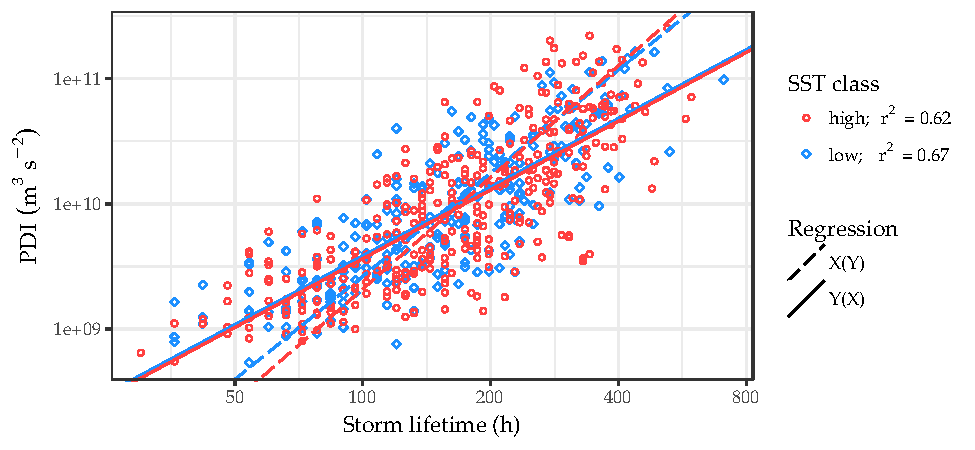
\includegraphics[width=\textwidth]{images/scatterplot-natl}
	\caption{Scatterplot of the joint distribution and regression analysis for the $PDI$ and lifetime of storms for the North Atlantic basin}
	\label{fig:natl-scatterplot}
\end{figure}

\begin{table}[H]
	\centering
	\begin{tabular}{cccccc}
		\toprule
		\toprule
		$X$ & $Y$ & SST class & $\hat{\beta}_{0}$ & $\hat{\beta}_{1}$ & $R^{2}$ \\
		\midrule
		\multirow{2}{*}{lifetime} & \multirow{2}{*}{$PDI$}
		 & Low  & \num{ 5.94 \pm 0.18} & \num{1.82 \pm 0.08} & \num{0.67} \\ % \pm 0.05} \\
		&& High & \num{ 5.91 \pm 0.17} & \num{1.83 \pm 0.08} & \num{0.62} \\ % \pm 0.04} \\
		\midrule
		\multirow{2}{*}{$PDI$} & \multirow{2}{*}{lifetime}
		 & Low  & \num{-1.44 \pm 0.16} & \num{0.37 \pm 0.02} & \num{0.67} \\ % \pm 0.05} \\
		&& High & \num{-1.14 \pm 0.14} & \num{0.34 \pm 0.01} & \num{0.62} \\ % \pm 0.04} \\
		\bottomrule
	\end{tabular}
	\caption{Linear regression coefficients obtained performing OLS on the North Atlantic basin data}
	\label{tab:natl-ols-coefs}
\end{table}

% The value of the studied statistics $T^{(i)}$ obtained from the N.~Atl. data set can be seen in \Cref{tab:base-natl-ols-statistics}.
\begin{table}[H]
	\centering
	\begin{tabular}{cccccccc}
	\toprule
	\toprule
	$X$   & $Y$   & $T^{(1)}$ & $T^{(2)}$ & $T^{(3)}$ & $T^{(4)}$ & $T^{(5)}$ & $T^{(6)}$ \\
	\midrule
	lifetime & $PDI$ & $0.025$ & $0.001$ & $0.051$ & $0.101$ & $0.010$ & $0.111$ \\
	$PDI$ & lifetime & $0.299$ & $0.028$ & $0.051$ & $1.388$ & $1.295$ & $2.683$ \\
	\bottomrule
	\end{tabular}
	\caption{Value of the test statistics for North Atlantic basin data set using OLS}
	\label{tab:base-natl-ols-statistics}
\end{table}

\bigskip
For the Northeast Pacific we have a similar situation. In \Cref{fig:epac-scatterplot} we can see the regression models that fit the joint bivariate lognormal distributions; the coefficient estimates obtained for each of these four resulting regression models are shown in \Cref{tab:epac-ols-coefs}. The values of the test statistics for this basin are shown in \Cref{tab:base-epac-ols-statistics}.


\medskip
We can see that the regressions for low-SST years and high-SST years are statistically compatible as well (\Cref{tab:epac-ols-coefs}). As it also happens for the North Atlantic, for the $PDI(\text{lifetime})$ regression the coefficients seem to be much closer, as can be clearly seen in \Cref{fig:epac-scatterplot}.

The results shown in \Cref{tab:base-epac-ols-statistics} are definitely surprising, in particular the value of $T^{(1)}$ for the $PDI(\text{lifetime}$ regression, as we expect this value to be smaller from theory. How much smaller, however, is not something we can calculate or predict from theory.

\begin{figure}[H]
	\centering
	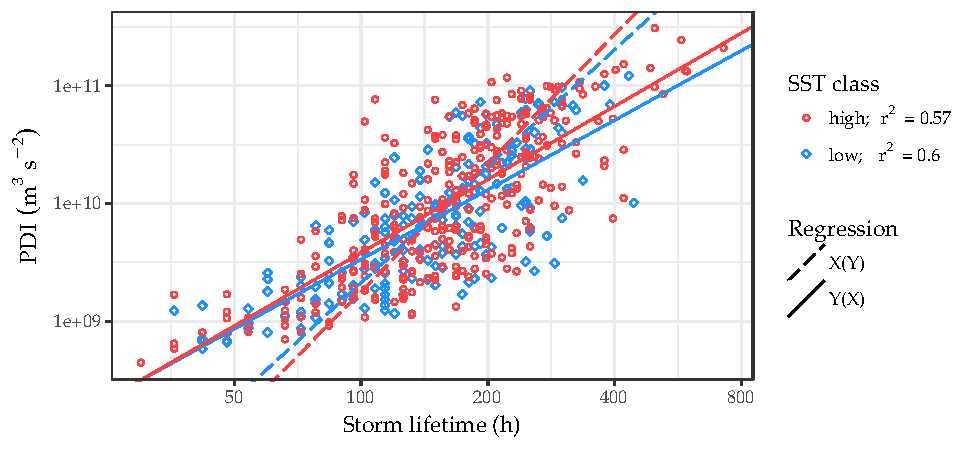
\includegraphics[width=\textwidth]{images/scatterplot-epac}
	\caption{Scatterplot of the joint distribution and regression analysis for the $PDI$ and lifetime of storms for the Northeast Pacific basin}
	\label{fig:epac-scatterplot}
\end{figure}

\begin{table}[H]
	\centering
	\begin{tabular}{cccccc}
		\toprule
		\toprule
		$X$ & $Y$ & SST class & $\hat{\beta}_{0}$ & $\hat{\beta}_{1}$ & $R^{2}$ \\
		\midrule
		\multirow{2}{*}{lifetime} & \multirow{2}{*}{$PDI$}
		 & Low  & \num{ 5.59 \pm 0.25} & \num{1.97 \pm 0.12} & \num{0.60} \\ % \pm 0.05} \\
		&& High & \num{ 5.45 \pm 0.23} & \num{2.07 \pm 0.10} & \num{0.57} \\ % \pm 0.04} \\
		\midrule
		\multirow{2}{*}{$PDI$} & \multirow{2}{*}{lifetime}
		 & Low  & \num{-0.83 \pm 0.18} & \num{0.30 \pm 0.02} & \num{0.60} \\ % \pm 0.05} \\
		&& High & \num{-0.55 \pm 0.14} & \num{0.28 \pm 0.01} & \num{0.57} \\ % \pm 0.04} \\
		\bottomrule
	\end{tabular}
	\caption{Linear regression coefficients obtained performing OLS on the Northeast Pacific basin data}
	\label{tab:epac-ols-coefs}
\end{table}

\begin{table}[H]
	\centering
	\begin{tabular}{cccccccc}
	\toprule
	\toprule
	$X$   & $Y$   & $T^{(1)}$ & $T^{(2)}$ & $T^{(3)}$ & $T^{(4)}$ & $T^{(5)}$ & $T^{(6)}$ \\
	\midrule
	lifetime & $PDI$ & $0.149$ & $0.103$ & $0.027$ & $0.437$ & $0.661$ & $1.099$ \\
	$PDI$ & lifetime & $0.285$ & $0.028$ & $0.027$ & $1.273$ & $1.254$ & $2.527$ \\
	\bottomrule
	\end{tabular}
	\caption{Value of the test statistics for Northeast Pacific basin data set using OLS}
	\label{tab:base-epac-ols-statistics}
\end{table}

\newpage
%-----------------------------------------------------------------
%	BOOTSTRAP: TESTING THE ASSUMPTIONS
%	!TEX root = ./../main.tex
%-----------------------------------------------------------------
\subsection{Testing the linear regression assumptions}\label{ssec:testing-assumptions}
As stated in \Cref{sec:simple-regression}, in linear regression the standard errors and hypothesis tests associated with the linear model rely on the random error $\epsilon$ being normal, independent, and homoscedastic.

Therefore, to be sure the results found on \Cref{sec:reg-analysis-data} are reliable, we should test these assumptions using the regression diagnostic tools introduced in \Cref{sec:reg-analysis-issues}. First we will analyse the North Atlantic basin data, and then we will analyse the Northeast Pacific basin data.

\bigskip
The first step is to have a look at the diagnostic plots. The diagnostic plots for the North Atlantic basin, separating the data by SST class can be observed in \Cref{fig:natl_residuals}.
\begin{figure}[H]
	\centering
	\subfloat[Q-Q plot (low SST)]{%
		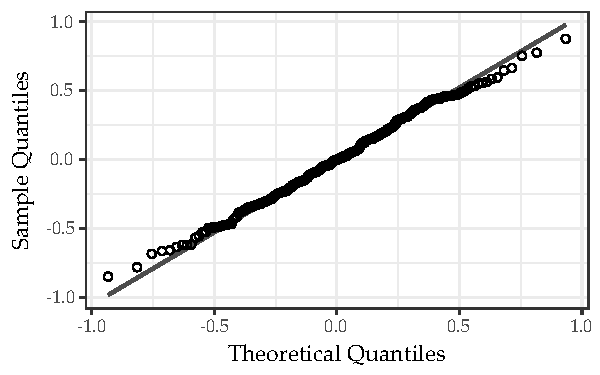
\includegraphics[width=0.45\textwidth]{./images/natl_low_resid_qqplot}
		\label{fig:natl_low_resid_qqplot}%
		}%
	\subfloat[Residuals vs fitted (low SST)]{%
		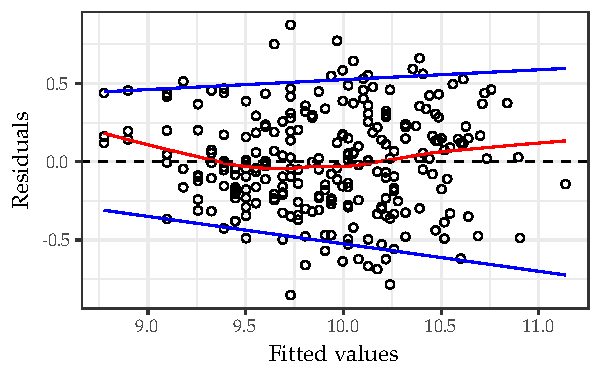
\includegraphics[width=0.45\textwidth]{./images/natl_low_resid_fitted}
		\label{fig:natl_low_resid_fitted}%
		}%
	\\
	\subfloat[Q-Q plot (high SST)]{%
		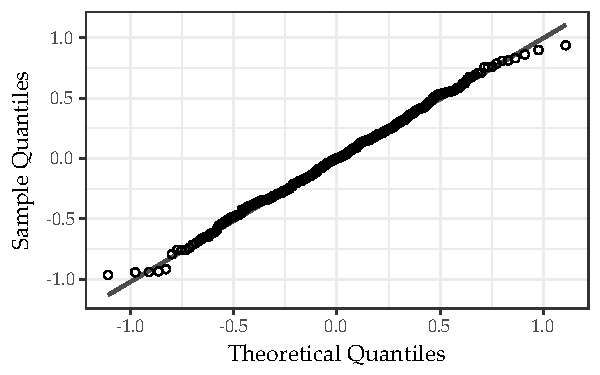
\includegraphics[width=0.45\textwidth]{./images/natl_high_resid_qqplot}
		\label{fig:natl_high_resid_qqplot}%
		}%
	\subfloat[Residuals vs fitted (high SST)]{%
		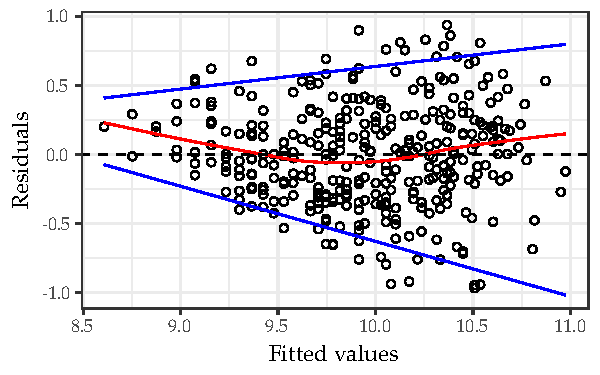
\includegraphics[width=0.45\textwidth]{./images/natl_high_resid_fitted}
		\label{fig:natl_high_resid_fitted}%
		}%
	\caption{Diagnostic plots to analyse the residuals for the North Atlantic basin}
	\label{fig:natl_residuals}
\end{figure}
In the Q-Q plots shown in \Cref{fig:natl_low_resid_qqplot} and \Cref{fig:natl_high_resid_qqplot} we can see that the residuals are mostly normal; if anything, the distribution has light tails. The residual plots in \Cref{fig:natl_low_resid_fitted} and \Cref{fig:natl_high_resid_fitted}, however, tell show us gross heteroscedasticity, specially for high-SST years.

To confirm this numerically, let us explore the results of performing the Lilliefors, correlation, and Breusch--Pagan tests for the North Atlantic basin in \Cref{tab:stat-tests-natl}.
\begin{table}[H]
	\centering
	\begin{tabular}{lccc}
		\toprule
		\toprule
		Data     & Lilliefors   & Correlation  & Breusch--Pagan \\
		\midrule
		Low-SST  & \num{0.7416} & \num{1.0000} & \num{0.0376}   \\
		High-SST & \num{0.9740} & \num{1.0000} & \num{0.0002}   \\
		\bottomrule
	\end{tabular}
	\caption{List of $p$-values associated with the statistical hypothesis tests to respectively analyse normality, independence, and homoscedasticity of the residuals on the low-SST and high-SST subsets of the North Atlantic basin}
	\label{tab:stat-tests-natl}
\end{table}
The $p$-values tell us that the only rejected hypothesis is homoscedasticity for both datasets, which is precisely what we observed on the residual plots.

\bigskip
For the Northeast Pacific basin we see a similar picture. The diagnostic plots for the this basin, separating the data by SST class can be observed in \Cref{fig:epac_residuals}.
\begin{figure}[H]
	\centering
	\subfloat[Q-Q plot (low SST)]{%
		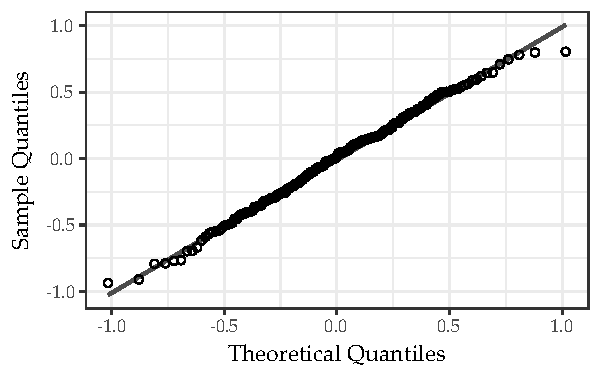
\includegraphics[width=0.45\textwidth]{./images/epac_low_resid_qqplot}
		\label{fig:epac_low_resid_qqplot}%
		}%
	\subfloat[Residuals vs fitted (low SST)]{%
		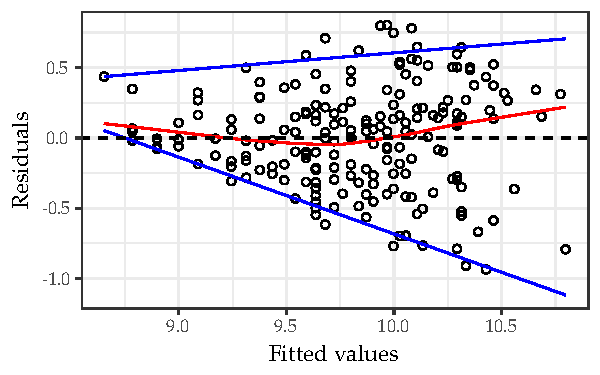
\includegraphics[width=0.45\textwidth]{./images/epac_low_resid_fitted}
		\label{fig:epac_low_resid_fitted}%
		}%
	\\
	\subfloat[Q-Q plot (high SST)]{%
		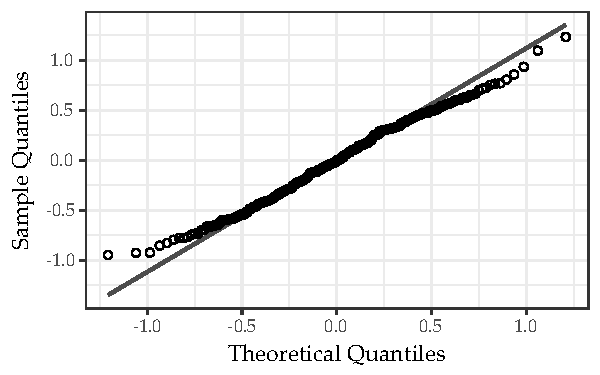
\includegraphics[width=0.45\textwidth]{./images/epac_high_resid_qqplot}
		\label{fig:epac_high_resid_qqplot}%
		}%
	\subfloat[Residuals vs fitted (high SST)]{%
		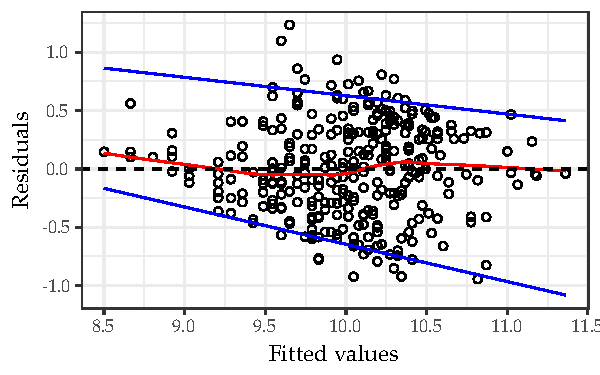
\includegraphics[width=0.45\textwidth]{./images/epac_high_resid_fitted}
		\label{fig:epac_high_resid_fitted}%
		}%
	\caption{Diagnostic plots to analyse the residuals for the Northeast Pacific basin}
	\label{fig:epac_residuals}
\end{figure}
In the Q-Q plot shown in \Cref{fig:epac_low_resid_qqplot} we can see that the residuals for low-SST year follow a normal distribution with light tails. The Q-Q plot for high-SST years shown in \Cref{fig:epac_high_resid_qqplot}, however, is strongly non-normal. The residual plots in \Cref{fig:epac_low_resid_fitted} and \Cref{fig:epac_high_resid_fitted} tell show us quite heteroscedastic residuals, specially for low-SST years.

Again, to confirm this numerically, we explore the results of performing the Lilliefors, correlation, and Breusch--Pagan tests for the Northeast Pacific basin seen in \Cref{tab:stat-tests-epac}.
\begin{table}[H]
	\centering
	\begin{tabular}{lccc}
		\toprule
		\toprule
		Data     & Lilliefors   & Correlation  & Breusch--Pagan \\
		\midrule
		Low-SST  & \num{0.7106} & \num{1.0000} & \num{0.0000}   \\
		High-SST & \num{0.0217} & \num{1.0000} & \num{0.1974}   \\
		\bottomrule
	\end{tabular}
	\caption{List of $p$-values associated with the statistical hypothesis tests to respectively analyse normality, independence, and homoscedasticity of the residuals on the low-SST and high-SST subsets of the Northeast Pacific basin}
	\label{tab:stat-tests-epac}
\end{table}
In this case, for low-SST years the rejected hypothesis is homoscedasticity, while for the high-SST years normality is the rejected hypothesis. This is precisely what we observed on the residual plots.

\bigskip
Having heteroscedasticity and non-normality tells us we cannot fully rely on the calculated standard errors, and we need to use bootstrap to obtain a more robust linear model to be able to infer statistical properties of the data using linear regression as the underlying model.

\newpage
%-----------------------------------------------------------------
%	BOOTSTRAP: RESAMPLING CASES
%	!TEX root = ./../main.tex
%-----------------------------------------------------------------
\subsection{Analysis using bootstrap}\label{sec:bootstrap}
We saw in \Cref{ssec:testing-assumptions} that some of the assumptions for the residual errors $\epsilon_{i}$ in the linear regression do not hold neither for the North Atlantic nor for the Northeast Pacific basins. It is for this reason that we use the bootstrapping methodology explained in \Cref{ssec:boot-theory} to resample the observations in order to obtain coefficient estimates $\hat{\beta}_{0}$, $\hat{\beta}_{1}$, and $R^{2}$ robust to failure of the model assumptions.

The particular implementation of \Cref{alg:bootstrap-theory} for our data can be seen in \Cref{alg:bootstrap}. The number of simulations performed in the bootstrap algorithm is $R = 500$ for each SST class.

\IncMargin{1em}
\begin{algorithm}[H]
	\caption{Bootstrap applied to linear regression}
	\label{alg:bootstrap}
	\DontPrintSemicolon
	\SetKwFunction{LinearModel}{LinearModel}
	\SetKwFunction{SubSet}{SubSet}
	\SetKwFunction{GetIntercept}{GetIntercept}
	\SetKwFunction{GetInterceptStdError}{GetInterceptStdError}
	\SetKwFunction{GetSlope}{GetSlope}
	\SetKwFunction{GetSlopeStdError}{GetSlopeStdError}
	\SetKwFunction{GetRSquared}{GetRSquared}
	\SetKwFunction{ResampleWithReplacement}{ResampleWithReplacement}
		\KwData{Hurricane observational data $O$, with paired variables $X$, $Y$; classified by SST class ($C : \qty{low ,high}$), with $n$ and $m$ observations respectively}
		\KwResult{Bootstrapped data for coefficient estimates for each SST class}
		% initialization\;
		\For{$class$ \textbf{in} $C$}{
			$O'$ $\gets$ \SubSet($(x,y) \in O \mid c \equiv class$)\;
			fit                    $\gets$ \LinearModel($Y' \sim X'$)\;
			$\hat{\beta}_{0}$      $\gets$ \GetIntercept(fit)\;
			$\hat{\beta}_{1}$      $\gets$ \GetSlope(fit)\;
			$R^2$                  $\gets$ \GetRSquared(fit)\;
			Initialise empty vectors $\va{\beta}_{0}^{\ast}$, $\va{\beta}_{1}^{\ast}$, $\va{R}^{2\ast}$ \;
			\For{$i \gets 1$ \textbf{to} $R$}{
				$O'^{\ast}$ $\gets$ \ResampleWithReplacement($O'$) \;
				fit$^{\ast}$                $\gets$ \LinearModel($Y'^{\ast} \sim X'^{\ast}$)  \;
				$\va{\beta}_{0}^{\ast}[i]$ $\gets$ \GetIntercept(fit$^{\ast}$) \;
				$\va{\beta}_{1}^{\ast}[i]$ $\gets$ \GetSlope(fit$^{\ast}$)     \;
				$\va{R}^{2\ast}[i]$              $\gets$ \GetRSquared(fit$^{\ast}$)  \;
			}
		}
		\Return{($\va{\beta}_{0, low}^{\ast}$, $\va{\beta}_{1, low}^{\ast}$, $\va{R}^{2\ast}_{low}$) \& ($\va{\beta}_{0, high}^{\ast}$, $\va{\beta}_{1, high}^{\ast}$, $\va{R}^{2\ast}_{high}$)} \;
\end{algorithm}
\DecMargin{1em}

This resampling algorithm is performed both for the $PDI(\text{lifetime})$ regression model as well as the inverse $\text{lifetime}(PDI)$ model.

\bigskip
To obtain the bootstrapped coefficient estimates $\hat{\beta}_{0}^{\ast}$, $\hat{\beta}_{1}^{\ast}$, $R^{2\ast}$, and and their associated standard errors from the resulting vector data $\va{\beta}_{0}^{\ast}$, $\va{\beta}_{1}^{\ast}$, and $\va{R}^{2\ast}$, one can simply calculate the mean and the standard deviation of their distributions:
\begin{align}
	\hat{\theta}^{\ast} = \frac{1}{R} \sum_{i=1}^{R} \theta_{i}
	\qc
	\se{\hat{\theta}^{\ast}}^{2} = \frac{1}{R} \sum_{i=1}^{R-1} \qty(\theta_{i} - \hat{\theta}^{\ast})^{2}
	.
\end{align}

This is possible because the bootstrapped data for estimating a coefficient $\theta$ (either $\beta_{0}$, $\beta_{1}$, or $R^{2}$) follows a normal distribution:
\begin{align}
	\va{\theta^{\ast}} \sim \mc{N}(\hat{\theta}^{\ast}, \se{\hat{\theta}^{\ast}}^{2} )
	.
\end{align}

%-----------------------------------------------------------------
% \subsubsection*{Resampled coefficients}
We can see this for the North Atlantic basin data in \Cref{fig:natl-boot-coefs}, where we plot the histograms of the bootstrapped intercept and slopes (both for low-SST and high-SST years), as well as a Q-Q plot to compare both distributions. Notice we only show these plots are only for the $PDI(\text{lifetime})$ regression model; for the inverse regression, the results and conclusions are comparable.

From \Cref{fig:natl-boot-inter} and \Cref{fig:natl-boot-slope} we can see how the bootstrap ensures the normality in the coefficients; this is also confirmed by the Q-Q plots in \Cref{fig:natl-boot-inter-qq} and \Cref{fig:natl-boot-slope-qq}, that show that the coefficients for different SST class are from the same distribution family (in this case, a normal). This ensures the assumptions in linear regression hold.

\begin{figure}[H]
	\centering
	\subfloat[Histogram of the bootstrapped intercept]{%
		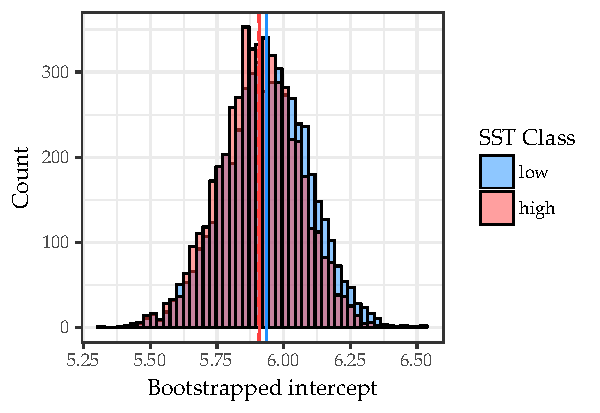
\includegraphics[width=0.45\textwidth]{./images/natl_boot_inter}
		\label{fig:natl-boot-inter}%
		}%
	\subfloat[Q-Q plot to compare the intercepts]{%
		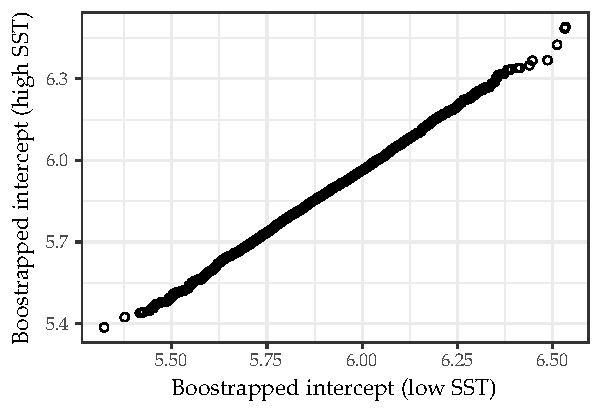
\includegraphics[width=0.45\textwidth]{./images/natl_boot_inter_qq}
		\label{fig:natl-boot-inter-qq}%
		}%
	\\
	\subfloat[Histogram of the bootstrapped slope]{%
		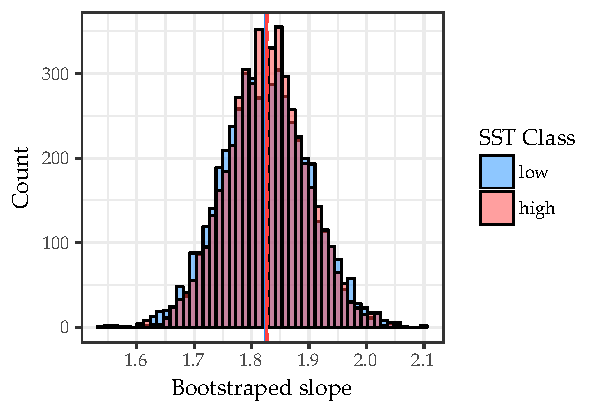
\includegraphics[width=0.45\textwidth]{./images/natl_boot_slope}
		\label{fig:natl-boot-slope}%
		}%
	\subfloat[Q-Q plot to compare the slopes]{%
		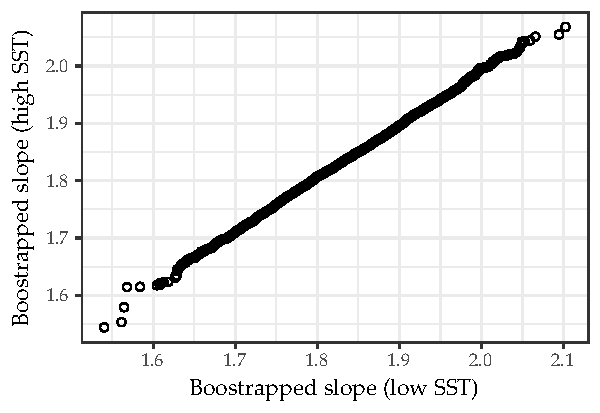
\includegraphics[width=0.45\textwidth]{./images/natl_boot_slope_qq}
		\label{fig:natl-boot-slope-qq}%
		}%
	\caption[Resampled slopes and intercepts obtained by bootstrapping for the North Atlantic basin data for the $PDI(\text{lifetime})$ regression model]{Resampled slopes and intercepts obtained by bootstrapping for the North Atlantic basin data for the $PDI(\text{lifetime})$ regression model. The dashed lines represent the coefficient estimates obtained via bootstrap, while the solid lines the estimates obtained via OLS}
	\label{fig:natl-boot-coefs}
\end{figure}

The coefficient estimates obtained for each of the four resulting regression models for the North Atlantic data are shown in \Cref{tab:natl-boot-coefs}. When compared to \Cref{tab:natl-ols-coefs} (coefficients obtained using OLS), one sees that the nominal values, as well as their standard error are almost identical.

This is by no means a bad thing. The main point of using bootstrap to resample the observations of hurricane occurrences was to have a robust theory to ensure the assumptions required for the linear model hold.

\begin{table}[H]
	\centering
	\begin{tabular}{cccccc}
		\toprule
		\toprule
		$X$ & $Y$ & SST class & $\hat{\beta}_{0}^{\ast}$ & $\hat{\beta}_{1}^{\ast}$ & $R^{2\ast}$ \\
		\midrule
		\multirow{2}{*}{lifetime} & \multirow{2}{*}{$PDI$}
		 & Low  & \num{ 5.91 \pm 0.17} & \num{1.84 \pm 0.08} & \num{0.67 \pm 0.03} \\
		&& High & \num{ 5.90 \pm 0.15} & \num{1.83 \pm 0.07} & \num{0.61 \pm 0.03} \\
		\midrule
		\multirow{2}{*}{$PDI$} & \multirow{2}{*}{lifetime}
		 & Low  & \num{-1.44 \pm 0.15} & \num{0.36 \pm 0.02} & \num{0.67 \pm 0.03} \\
		&& High & \num{-1.15 \pm 0.14} & \num{0.34 \pm 0.01} & \num{0.62 \pm 0.03} \\
		\bottomrule
	\end{tabular}
	\caption{Linear regression coefficients obtained performing bootstrap on the North Atlantic basin data}
	\label{tab:natl-boot-coefs}
\end{table}

The values of the test statistics calculated using the coefficient estimates obtained using bootstrap for this basin are shown in \Cref{tab:base-natl-boot-statistics}. The results, save some small discrepancies in the $\text{lifetime}(PDI)$ regression model, are comparable to those displayed in \Cref{tab:base-natl-ols-statistics}.
\begin{table}[H]
	\centering
	\begin{tabular}{cccccccc}
	\toprule
	\toprule
	$X$   & $Y$   & $T^{(1)}$ & $T^{(2)}$ & $T^{(3)}$ & $T^{(4)}$ & $T^{(5)}$ & $T^{(6)}$ \\
	\midrule
	lifetime & $PDI$ & $0.007$ & $0.007$ & $0.054$ & $0.031$ & $0.065$ & $0.095$ \\
	$PDI$ & lifetime & $0.289$ & $0.027$ & $0.048$ & $1.404$ & $1.324$ & $2.727$ \\
	\bottomrule
	\end{tabular}
	\caption{~Value of the studied statistics for North Atlantic basin data set using bootstrap}
	\label{tab:base-natl-boot-statistics}
\end{table}

%-----------------------------------------------------------------
\bigskip
For the Northeast Pacific basin data, we also observe normality in the bootstrapped coefficients, as can be seen in \Cref{fig:epac-boot-coefs}. A major difference, that we did not see in \Cref{fig:natl-boot-coefs} is that the distributions associated to low-SST and high-SST years present very distinct shapes, but this is a result of the inherent properties of the data; it represents the same numerical difference we already saw in the OLS coefficient estimates shown in \Cref{tab:epac-ols-coefs}), but from a graphical point of view.

\begin{figure}[H]
	\centering
	\subfloat[Histogram of the bootstrapped intercept]{%
		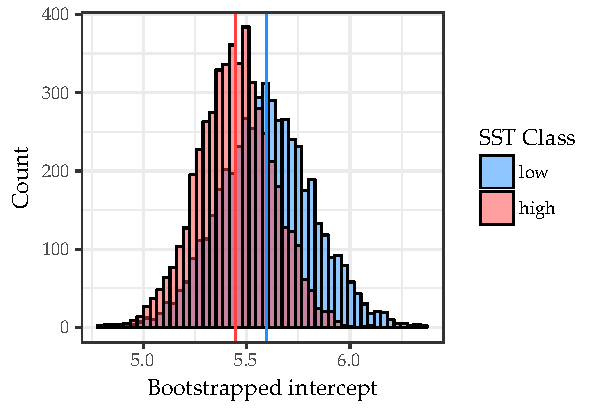
\includegraphics[width=0.45\textwidth]{./images/epac_boot_inter}
		\label{fig:epac-boot-inter}%
		}%
	\subfloat[Q-Q plot to compare the intercepts]{%
		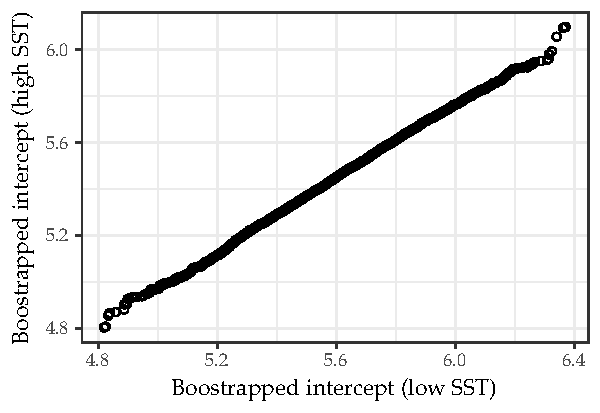
\includegraphics[width=0.45\textwidth]{./images/epac_boot_inter_qq}
		\label{fig:epac-boot-inter-qq}%
		}%
	\\
	\subfloat[Histogram of the bootstrapped slope]{%
		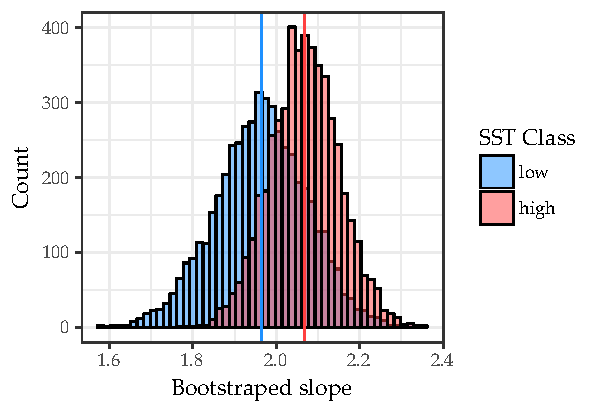
\includegraphics[width=0.45\textwidth]{./images/epac_boot_slope}
		\label{fig:epac-boot-slope}%
		}%
	\subfloat[Q-Q plot to compare the slopes]{%
		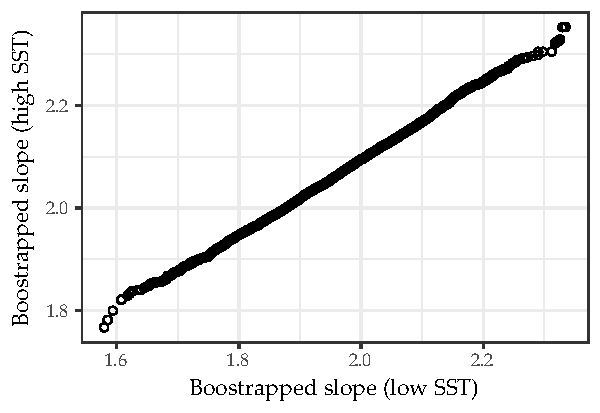
\includegraphics[width=0.45\textwidth]{./images/epac_boot_slope_qq}
		\label{fig:epac-boot-slope-qq}%
		}%
	\caption[Resampled slopes and intercepts obtained by bootstrapping for the Northeast Pacific basin data for the $PDI(\text{lifetime})$ regression model]{Resampled slopes and intercepts obtained by bootstrapping for the Northeast Pacific basin data for the $PDI(\text{lifetime})$ regression model. The dashed lines represent the coefficient estimates obtained via bootstrap, while the solid lines the estimates obtained via OLS}
	\label{fig:epac-boot-coefs}
\end{figure}

% \todo[inline]{Talk about coefficients of the linear regression}
The coefficient estimates obtained for each of the four resulting regression models for the Northeast Pacific data are shown in \Cref{tab:epac-boot-coefs}. When compared to \Cref{tab:epac-ols-coefs} (coefficients obtained using OLS), one sees that the nominal values, as well as their standard error are almost identical, just as happened for the North Atlantic data.

\begin{table}[H]
	\centering
	\begin{tabular}{cccccc}
		\toprule
		\toprule
		$X$ & $Y$ & SST class & $\hat{\beta}_{0}^{\ast}$ & $\hat{\beta}_{1}^{\ast}$ & $R^{2\ast}$ \\
		\midrule
		% \cmidrule(l){2-5}
		\multirow{2}{*}{lifetime} & \multirow{2}{*}{$PDI$}
		 & Low  & \num{ 5.59 \pm 0.24} & \num{1.97 \pm 0.12} & \num{0.60 \pm 0.05} \\
		&& High & \num{ 5.44 \pm 0.18} & \num{2.07 \pm 0.08} & \num{0.57 \pm 0.04} \\
		\midrule
		\multirow{2}{*}{$PDI$} & \multirow{2}{*}{lifetime}
		 & Low  & \num{-0.84 \pm 0.17} & \num{0.30 \pm 0.02} & \num{0.60 \pm 0.05} \\
		&& High & \num{-0.56 \pm 0.14} & \num{0.28 \pm 0.01} & \num{0.57 \pm 0.04} \\
		\bottomrule
	\end{tabular}
	\caption{Linear regression coefficients obtained performing bootstrap on the Northeast Pacific basin data}
	\label{tab:epac-boot-coefs}
\end{table}

The values of the test statistics calculated using the coefficient estimates obtained using bootstrap for this basin are shown in \Cref{tab:base-epac-boot-statistics}. The results are comparable and almost identical to those displayed in \Cref{tab:base-epac-ols-statistics}.

\begin{table}[H]
	\centering
	\begin{tabular}{cccccccc}
	\toprule
	\toprule
	$X$   & $Y$   & $T^{(1)}$ & $T^{(2)}$ & $T^{(3)}$ & $T^{(4)}$ & $T^{(5)}$ & $T^{(6)}$ \\
	\midrule
	lifetime & $PDI$ & $0.152$ & $0.103$ & $0.030$ & $0.509$ & $0.728$ & $1.237$ \\
	$PDI$ & lifetime & $0.286$ & $0.028$ & $0.027$ & $1.266$ & $1.266$ & $2.532$ \\
	\bottomrule
	\end{tabular}
	\caption{~Value of the studied statistics for Northeast Pacific basin data set using bootstrap}
	\label{tab:base-epac-boot-statistics}
\end{table}

\bigskip
% I summary, one can notice that the value of some of the $T^{(i)}$ statistics seem a bit high, both when performing a standard (OLS) regression analysis or a bootstrap-powered regression analysis. The problem is there is no way to quantify how big these statistics can be from theory.

% It is for this reason that we should perform a permutation test on the data following the methodology explained in \Cref{ssec:perm-test-theory}. This would allow us to properly test the hypothesis that
% \begin{align}
% 	f(Y \mid X = x)_{\text{low}} = f(Y \mid X = x)_{\text{high}}
% 	\tag{\ref{eq:hypothesis} ter}
% 	.
% \end{align}

\newpage
%-----------------------------------------------------------------
%	STATISTICAL HYPOTHESIS TESTING
%	!TEX root = ./../main.tex
%-----------------------------------------------------------------
\subsection{Analysis using permutation tests}\label{sec:perm-test}

In \Cref{sec:reg-analysis-data} and \Cref{sec:bootstrap} we noticed that the value of some of the $T^{(i)}$ statistics seem a bit high, both when performing a standard (OLS) regression analysis or a bootstrap-powered regression analysis. The problem is there is no way to quantify how big these statistics can be from theory.

It is for this reason that we should perform a permutation test on the data following the methodology explained in \Cref{ssec:perm-test-theory}. This would allow us to properly quantify the statistical significance of evidence against the hypothesis that storms of equal lifetime should, in theory, have the same wind speed and $PDI$, and have the same joint distribution, regardless of the SST.


\bigskip
The particular implementation of \Cref{alg:perm-test-theory} for our data can be seen in \Cref{alg:perm-test}. The number of simulations performed in the permutation test algorithm is $R = 1000$.

In the algorithm, $\text{fit}_{low/high}$ is an object that contains the coefficient estimates of the linear model. For the sake of robustness in the coefficient estimates calculated on each permutation, \texttt{LinearModel()} allows, as an option, to perform the estimations using bootstrap; the number of bootstrap simulations in these cases is $R' = 500$.

\IncMargin{1em}
\begin{algorithm}[H]
	\caption{Permutation test to compare two populations using linear regression}
	\label{alg:perm-test}
	\DontPrintSemicolon
	\SetKwFunction{LinearModel}{LinearModel}
	\SetKwFunction{GetStatistic}{GetStatistic}
	\SetKwFunction{Filter}{Filter}
	\SetKwFunction{SubSet}{SubSet}
	\SetKwFunction{Permute}{Permute}
		\KwData{Hurricane observational data $O$, with paired variables $X$, $Y$; classified by SST class ($C : \qty{low ,high}$), with $n$ and $m$ observations respectively}
		\KwResult{$p$-values defined under the null hypothesis}
		% initialization\;
		$O_{low}$ $\gets$ \SubSet($(x,y) \in O \mid c \equiv low$)\;
		$O_{high}$ $\gets$ \SubSet($(x,y) \in O \mid c \equiv high$)
		\tcp*{Notice that $O_{low} \cap O_{high} = O$}
		fit$_{low}$ $\gets$ \LinearModel($Y_{low} \sim X_{low}$) \;
		fit$_{high}$ $\gets$ \LinearModel($Y_{high} \sim X_{high}$)\;
		$T$ $\gets$ \GetStatistic(fit$_{low}$, fit$_{high}$) \;
		count = 0 \;
		\For{$i \gets 1$ \textbf{to} $R$}{
			$O'$ $\gets$ \Permute($O$) \;
			$O_{low}^{\ast}$ $\gets$ \SubSet($(x,y)_{i} \in O', \forall i \in [1, n]$ )\;
			$O_{high}^{\ast}$ $\gets$ \SubSet($(x,y)_{i} \in O', \forall i \in [n+1, n+m]$ )
			\tcp*{$O_{low}^{\ast} \cap O_{high}^{\ast} = O'$}
			fit$_{low}^{\ast}$ $\gets$ \LinearModel($Y_{low}^{\ast} \sim X_{low}^{\ast}$)\;
		fit$_{high}^{\ast}$ $\gets$ \LinearModel($Y_{high}^{\ast} \sim X_{high}^{\ast}$)\;
			$T^{\ast}$ $\gets$ \GetStatistic(fit$_{low}^{\ast}$, fit$_{high}^{\ast}$) \;
			\If{$T^{\ast} > T$}{
				count $\gets$ count + 1
			}
		}
		\Return{$p$-value $\gets$ count / $R$} \;
\end{algorithm}
\DecMargin{1em}

% The associated standard error to the $p$-value is defined as
% \begin{align}
% 	\se{p} = 1.96 \sqrt{\frac{p - p^{2}}{R}} ,
% \end{align}
% where $R$ is the number of simulations performed in the permutation test (\num{1000} in our case).

Notice that we only illustrate one test statistic in \Cref{alg:perm-test}; this is just to avoid overcomplicating the basic concept behind the permutation test. Naturally, in our case, we calculate all the test statistics proposed in section \Cref{sec:statistics-intro}:
\begin{align}
	T^{(1)} = \abs{\hat{\beta}_{0,h} - \hat{\beta}_{0,l}}
	\qc
	T^{(2)} = \abs{\hat{\beta}_{1,h} - \hat{\beta}_{1,l}}
	\qc
	T^{(3)} = \abs{ R^{2}_{h} - R^{2}_{l} }, \tag{\ref{eq:h0-stat-simple} bis}
\end{align}
\begin{align}
	T^{(4)} = \frac{\abs{\hat{\beta}_{0,h} - \hat{\beta}_{0,l}}}{\se{\hat{\beta}_{0,h} - \hat{\beta}_{0,l}}}
	\qc
	T^{(5)} = \frac{\abs{\hat{\beta}_{1,h} - \hat{\beta}_{1,l}}}{\se{\hat{\beta}_{1,h} - \hat{\beta}_{1,l}}}
	\qc
	T^{(6)} = T^{(4)} + T^{(5)} .
	\tag{\ref{eq:h0-stat-polko} bis}
\end{align}

%-----------------------------------------------------------------
In \Cref{tab:perm-natl-ols-p-vals} and \Cref{tab:perm-natl-boot-p-vals} we can see the $p$-values associated to each test statistic under the null hypothesis, using the standard OLS method and the bootstrap method, respectively, to calculate the coefficient estimates of the regression models for the North Atlantic basin data.

As we can see, neither of the tests rejects the null hypothesis, both using OLS and bootstrap as the underlying calculation for the model coefficient estimates. This indicates a strong evidence in favour of the null hypothesis being true.
\begin{table}[H]
	\centering
	\begin{tabular}{cccccccc}
	\toprule
	\toprule
	$X$  & $Y$       & $T^{(1)}$ & $T^{(2)}$ & $T^{(3)}$ & $T^{(4)}$ & $T^{(5)}$ & $T^{(6)}$ \\
	\midrule
	lifetime & $PDI$ & $0.164$ & $0.184$ & $0.749$ & $0.160$ & $0.187$ & $0.173$ \\
	% lifetime & $PDI$ & $0.176$   & $0.154$   & $0.740$   & $0.174$   & $0.148$   & $0.162$   \\
	$PDI$ & lifetime & $0.901$ & $0.991$ & $0.750$ & $0.900$ & $0.992$ & $0.968$ \\
	% $PDI$ & lifetime & $0.990$   & $0.930$   & $0.766$   & $0.990$   & $0.926$   & $0.972$   \\
	\bottomrule
	\end{tabular}
	\caption{List of $p$-values of the standard (OLS) permutation test for the North Atlantic basin data}
	\label{tab:perm-natl-ols-p-vals}
\end{table}

\begin{table}[H]
	\centering
	\begin{tabular}{cccccccc}
	\toprule
	\toprule
	$X$  & $Y$       & $T^{(1)}$ & $T^{(2)}$ & $T^{(3)}$ & $T^{(4)}$ & $T^{(5)}$ & $T^{(6)}$ \\
	\midrule
	lifetime & $PDI$ & $0.160$ & $0.187$ & $0.778$ & $0.132$ & $0.162$ & $0.142$ \\
	% lifetime & $PDI$ & $0.146$   & $0.121$   & $0.711$   & $0.137$   & $0.117$   & $0.128$   \\
	$PDI$ & lifetime & $0.925$ & $0.987$ & $0.757$ & $0.922$ & $0.995$ & $0.977$ \\
	% $PDI$ & lifetime & $0.870$   & $0.806$   & $0.705$   & $0.864$   & $0.795$   & $0.830$   \\
	\bottomrule
	\end{tabular}
	\caption{List of $p$-values of the bootstrap-powered permutation test for the North Atlantic basin data}
	\label{tab:perm-natl-boot-p-vals}
\end{table}


%-----------------------------------------------------------------
Similarly, for the Northeast Pacific basin, neither of the tests rejects the null hypothesis, both using OLS (\Cref{tab:perm-natl-ols-p-vals}) and bootstrap (\Cref{tab:perm-natl-boot-p-vals}) as the underlying calculation for the model coefficient estimates. This indicates a strong evidence in favour of the null hypothesis being true.
\begin{table}[H]
	\centering
	\begin{tabular}{cccccccc}
	\toprule
	\toprule
	$X$  & $Y$       & $T^{(1)}$ & $T^{(2)}$ & $T^{(3)}$ & $T^{(4)}$ & $T^{(5)}$ & $T^{(6)}$ \\
	\midrule
	lifetime & $PDI$ & $0.233$ & $0.232$ & $0.354$ & $0.243$ & $0.245$ & $0.247$ \\
	$PDI$ & lifetime & $0.629$ & $0.480$ & $0.329$ & $0.622$ & $0.475$ & $0.549$ \\
	\bottomrule
	\end{tabular}
	\caption{List of $p$-values of the standard (OLS) permutation test for the Northeast Pacific basin data}
	\label{tab:perm-epac-ols-p-vals}
\end{table}

\begin{table}[H]
	\centering
	\begin{tabular}{cccccccc}
	\toprule
	\toprule
	$X$  & $Y$       & $T^{(1)}$ & $T^{(2)}$ & $T^{(3)}$ & $T^{(4)}$ & $T^{(5)}$ & $T^{(6)}$ \\
	\midrule
	lifetime & $PDI$ & $0.250$ & $0.238$ & $0.365$ & $0.230$ & $0.231$ & $0.229$ \\
	$PDI$ & lifetime & $0.717$ & $0.533$ & $0.376$ & $0.721$ & $0.551$ & $0.632$ \\
	\bottomrule
	\end{tabular}
	\caption{List of $p$-values of the bootstrap-powered permutation test for the Northeast Pacific basin data}
	\label{tab:perm-epac-boot-p-vals}
\end{table}

\newpage

%-----------------------------------------------------------------
% \section{Regression analysis using permutation tests}\label{sec:regr-analysis-perm-test}
% %-----------------------------------------------------------------
%	BOOTSTRAP: CONCLUSIONS
%	!TEX root = ./../main.tex
%-----------------------------------------------------------------
\section{Conclusions}
In this work we have thoroughly explored and analysed the theoretical foundation of the linear regression under the ordinary least squares method. In particular, we saw both graphically and numerically how some of the assumptions on the random error, such as homoscedasticity and normality, do not hold for the joint distribution of $PDI$ and storm lifetime for the North Atlantic and Northeast Pacific basins.

To solve these problems, we used bootstrap to resample the observations in order to provide a more accurate and robust regression analysis than the one provided by the OLS method.

Last but not least, we proposed a statistical test to compare low-SST and high-SST years by performing a permutation test. This allowed us to quantify the statistical significance of evidence against the hypothesis that storms of equal lifetime have the same $PDI$ and same joint distribution, regardless of the SST. The results provide strong evidence that this hypothesis is indeed true, as none of the performed tests rejected the null hypothesis.

Our conclusions are compatible with the view of tropical cyclones as an activation process, in which, once the event has started, its intensity is kept in critical balance between attenuation and intensification (and so, higher SST does not trigger more intensification).

\bigskip
An open question, nonetheless, is why the increase of tropical-cyclone lifetime with SST triggers an increase in wind speed as a by-product.

The results of a simple exploratory analysis of the geographical properties of the tropical-cyclones show that the longer lifetimes for high-SST are mainly due to a shift to South-East of the tropical-cyclones genesis point, although further analysis is needed.

The steps to follow would be to perform a hierarchical clustering of the location of genesis and death of storms using the aggregate information provided by the $PDI$, lifetime, location, and path length of each storm to have a deeper understanding of the difference between hurricane occurrences in low-SST and high-SST years.

% %-----------------------------------------------------------------
%	PERMUTATION TESTS: CONCLUSIONS
%	!TEX root = ./../main.tex
%-----------------------------------------------------------------
\subsection{Conclusions}
\lipsum[1]


%-----------------------------------------------------------------
\section{Geographical analysis}\label{sec:geographical-analysis}
%-----------------------------------------------------------------
%	GEOGRAPHIC ANALYSIS
%	!TEX root = ./../main.tex
%-----------------------------------------------------------------

% \begin{itemize}
% 	\item Distance
% 	\item Linear regression?
% 	\item Analysis of initial/final position.
% 	\item Marginals of the finitial positions (4 plots per basin + summary).
% 	\item Boxplots and Wilcoxon tests.
% 	\item Clustering.
% \end{itemize}

\subsection{Geographical variables}
During the analysis performed in \Cref{sec:data-analysis} and \Cref{sec:regr-analysis-boot} we only used geographical information about the hurricane occurrences for the calculation of the basin-wide averaged SST.

From the raw HURDAT2 data sets, we can extract some relevant geographical data about each tropical-cyclone that could help obtain some insight or physical reason behind the displacement of the joint distribution of $PDI$ and lifetime of the storms between low-SST and high-SST years occurrences.

\bigskip
We focus on the geographical genesis location of a tropical-cyclone, as well as its death location. This information is easy to get from the individual longitude and latitude tracks for each hurricane.

Apart from this, we calculate the total travelled distance, or path length, of each hurricane by means of the \emph{spherical law of cosines}:
\begin{align}
	d(p_{1}, p_{2}) = \cos^{-1}\qty[\sin(\phi_{1}) \cdot \sin(\phi_{2}) + \cos(\phi_{1}) \cdot \cos(\phi_{2}) \cdot \cos(\Delta \lambda)] \cdot R_{\text{E}},
\end{align}
where $\phi$ and $\lambda$ respectively represent latitude and longitude in radians, and $R_{\text{E}}$ represents the Earth's radius in meters.

\medskip
In \Cref{hd:geog-data-head} one can see the structure of the cleaned data illustrate these newly calculated geographical variables.
\begin{table}[H]
	\centering
	\ttfamily
	\resizebox{\textwidth}{!}{%
	\begin{tabular}{r r r r c r r r r r}
		\toprule
		\toprule
		storm.id & storm.name & n.obs & storm.duration & \multirow{2}{*}{$\cdots$} & first.lat & last.lat & first.long & last.long &  distance \\
		<chr>    & <chr>      & <int> &          <dbl> &          &     <dbl> &    <dbl> &      <dbl> &     <dbl> &     <dbl> \\
		\midrule
		AL011966 & ALMA       &    42 &         907200 & $\cdots$ &      12.7 &     42.0 &      -84.0 &     -70.5 &   4129705 \\
		AL021966 & BECKY      &     9 &         194400 & $\cdots$ &      32.4 &     45.5 &      -57.8 &     -58.5 &   1678458 \\
		AL031966 & CELIA      &    36 &         777600 & $\cdots$ &      19.1 &     52.0 &      -59.5 &     -57.0 &   5635625 \\
		AL041966 & DOROTHY    &    37 &         799200 & $\cdots$ &      31.0 &     53.5 &      -41.0 &     -38.5 &   2864172 \\
		AL051966 & ELLA       &    26 &         561600 & $\cdots$ &      10.0 &     24.3 &      -35.0 &     -68.4 &   3917529 \\
		AL071966 & GRETA      &    26 &         561600 & $\cdots$ &      13.7 &     28.0 &      -48.4 &     -71.7 &   2977350 \\
		\bottomrule
	\end{tabular}}
	\caption{Excerpt of the North Atlantic data set, focusing on the geographical variables}
	\label{hd:geog-data-head}
\end{table}

\bigskip
Similarly to the unified HURDAT2 \& HadISST1 data sets (see \Cref{ssec:unified-data-set}), these geographically enhanced data sets are available in the \texttt{HurdatHadISSTData} package:
\begin{itemize}
	\item \texttt{tc.pdi.geog.natl} -- Data set for the North Atlantic basin.
	\item \texttt{tc.pdi.geog.epac} -- Data set for the Northeast Pacific basin.
	\item \texttt{tc.pdi.geog.all} -- Data set for both basins.
\end{itemize}

\newpage
%-----------------------------------------------------------------
%	GEOGRAPHIC ANALYSIS
%	!TEX root = ./../main.tex
%-----------------------------------------------------------------
\subsection{Analysis of the path length}
In \Cref{fig:natl-distance-bvln} and \Cref{fig:epac-distance-bvln} we can see the bivariate lognormal distributions of the path length $d$ and lifetime of the storms for the North Atlantic and Northeast Pacific basins separating storms by SST class.

\begin{figure}[H]
	\centering
	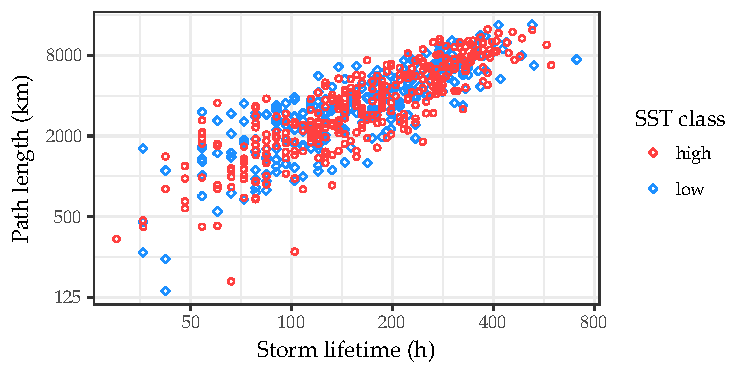
\includegraphics[width=0.8\textwidth]{images/natl-distance-bvln}
	\caption{Bivariate lognormal distribution $f(d, \text{lifetime})$ of the hurricane observations for the North Atlantic basin}
	\label{fig:natl-distance-bvln}
\end{figure}

\begin{figure}[H]
	\centering
	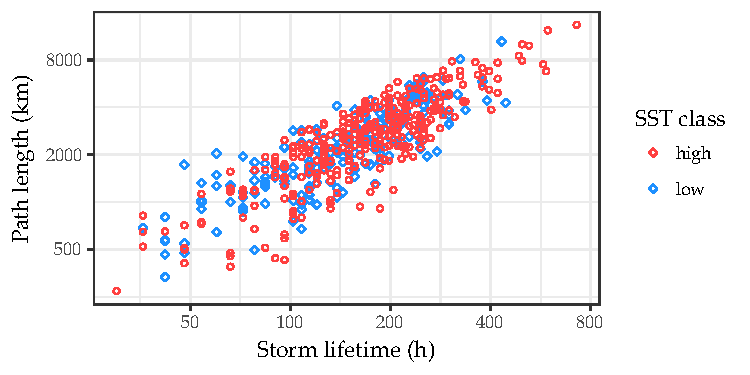
\includegraphics[width=0.9\textwidth]{images/epac-distance-bvln}
	\caption{Bivariate lognormal distribution $f(d, \text{lifetime})$ of the hurricane observations for the Northeast Pacific basin}
	\label{fig:epac-distance-bvln}
\end{figure}

Contrarily to the procedure of analysing the marginals of this joint distribution that we performed on \Cref{ssec:univariate}, we want study the mean focus on the forward speed of the hurricanes. Notice that this speed is different to the sustained surface
wind speed. Naturally, this mean forward speed is calculated as
\begin{align}
	\ev{v_{f}} = \frac{d}{\text{lifetime}} .
\end{align}
We think this variable may be an intermediary variable to relate the storm path length and its $PDI$, and expect a displacement to higher speeds for high-SST years.

\medskip
In \Cref{fig:natl-forward-speed} we show a histogram of the mean forward speed for the North Atlantic basin, while in \Cref{fig:epac-forward-speed} we show the same histogram for the Northeast Pacific basin.

As it can be seen, there seems to be no general trend on the behaviour of the mean forward between the North Atlantic and Northeast Pacific basins.
\begin{figure}[H]
	\centering
	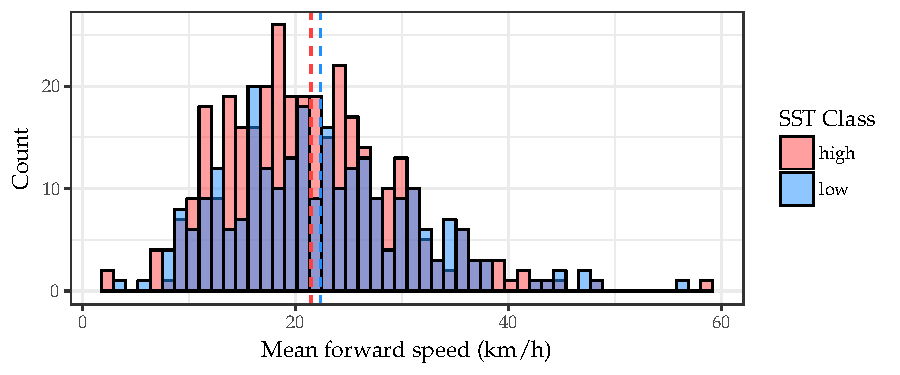
\includegraphics[width=0.9\textwidth]{images/natl-forward-speed}
	\caption{Mean forward speed histogram for the North Atlantic basin}
	\label{fig:natl-forward-speed}
\end{figure}

\begin{figure}[H]
	\centering
	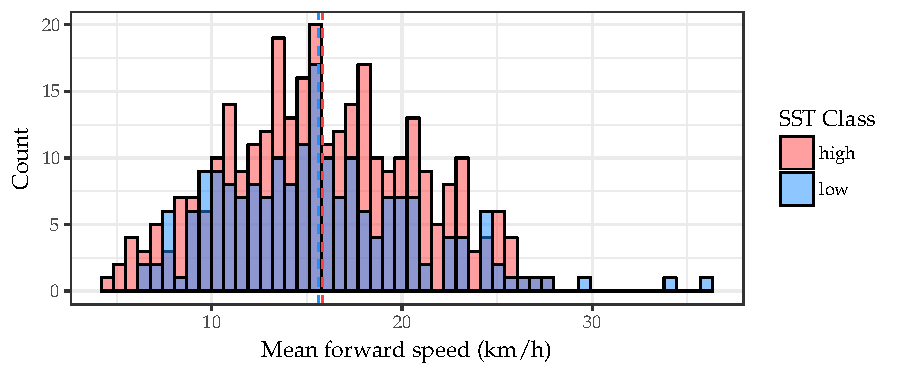
\includegraphics[width=0.8\textwidth]{images/epac-forward-speed}
	\caption{Mean forward speed histogram for the Northeast Pacific basin}
	\label{fig:epac-forward-speed}
\end{figure}

\newpage
%-----------------------------------------------------------------
%	GEOGRAPHIC ANALYSIS
%	!TEX root = ./../main.tex
%-----------------------------------------------------------------
\subsection{Analysis of the location}
A particularly important variable in this analysis is, obviously, the location of genesis of the storms, and possibly their location of death.

In this part we do an exploratory comparison of the difference in position of genesis and death of tropical-cyclones between low-SST and high-SST years.

\medskip
In \Cref{fig:natl-positions} we can see the distributions of genesis and death positions (longitude and latitde) of the storms occurred on the North Atlantic basin, while in \Cref{tab:natl-positions} we can see the expected value of the distributions.

The results suggest show the major difference between low-SST and high-SST years is the location of the genesis of the hurricanes, as it seems to be displaced to the South-East. However, there is no significant difference in the death location.
\begin{figure}[H]
	\centering
	\subfloat[Distribution of the genesis longitude]{%
		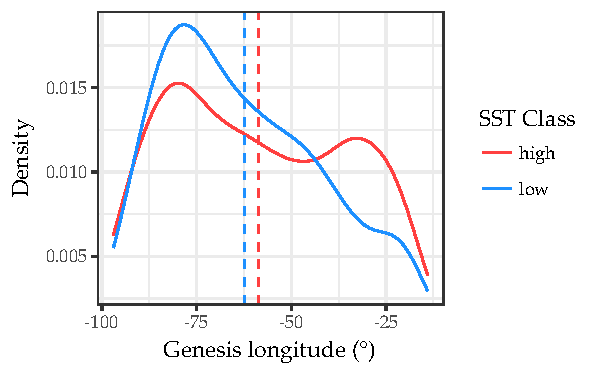
\includegraphics[width=0.5\textwidth]{./images/natl-init-long}
		\label{fig:images/natl-init-long}%
		}%
	\subfloat[Distribution of the death longitude]{%
		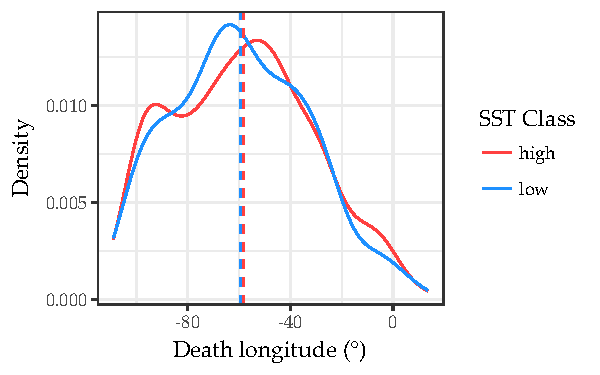
\includegraphics[width=0.5\textwidth]{./images/natl-final-long}
		\label{fig:images/natl-final-long}%
		}%
	\\
	\subfloat[Distribution of the genesis latitude]{%
		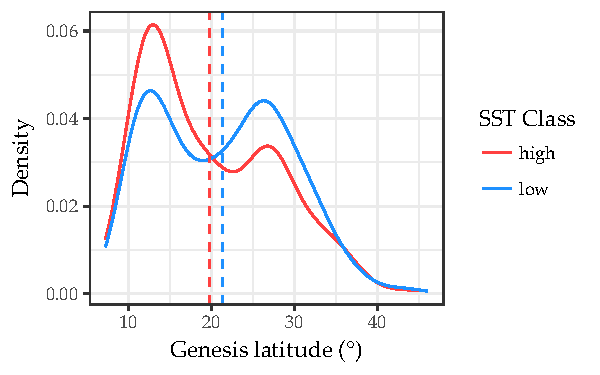
\includegraphics[width=0.5\textwidth]{./images/natl-init-lat}
		\label{fig:images/natl-init-lat}%
		}%
	\subfloat[Distribution of the death latitude]{%
		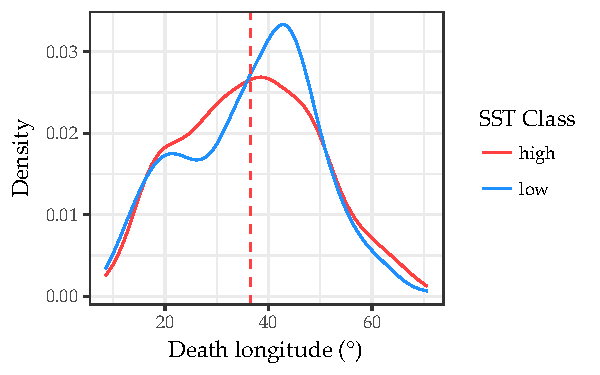
\includegraphics[width=0.5\textwidth]{./images/natl-final-lat}
		\label{fig:images/natl-final-lat}%
		}%
	\caption{Spatial distributions of the geographical position variables of storms for the North Atlantic basin}
	\label{fig:natl-positions}
\end{figure}

\begin{table}[H]
	\centering
	\begin{tabular}{c cc cc}
		\toprule
		\toprule
		SST Class & $\bar{\lambda}_{\text{gen}}$   & $\bar{\phi}_{\text{gen}}$
		          & $\bar{\lambda}_{\text{death}}$ & $\bar{\phi}_{\text{death}}$ \\
		\midrule
		Low       & \num{-59.35 \pm 22.94} & \num{20.84 \pm 7.97} & \num{-59.37 \pm 24.09} & \num{33.08 \pm 12.94} \\
		High      & \num{-58.68 \pm 23.44} & \num{19.47 \pm 7.74} & \num{-59.39 \pm 26.57} & \num{34.72 \pm 13.31} \\
		\bottomrule
	\end{tabular}
	\caption{Summary of the expected values of the geographical position variables of storms for the North Atlantic basin}
	\label{tab:natl-positions}
\end{table}

%-----------------------------------------------------------------
For the Northeast Pacific we have a similar scenario. In \Cref{fig:epac-positions} we can see the distributions of genesis and death positions (longitude and latitde) of the storms, while in \Cref{tab:epac-positions} we can see the expected value of the distributions.

The results suggest show the major difference between low-SST and high-SST years is the location of the genesis of the hurricanes, as it seems to be displaced to the South-East. Contrarily to the North Atlantic, in the Northeast Pacific, there seems to be a slight displacement in the death position for high-SST years to the North-East.

\begin{figure}[H]
	\centering
	\subfloat[Distribution of the genesis longitude]{%
		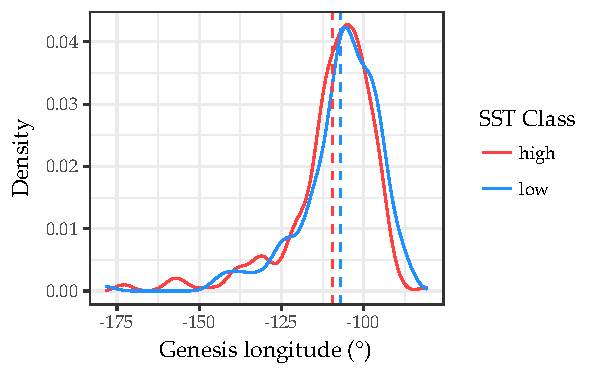
\includegraphics[width=0.5\textwidth]{./images/epac-init-long}
		\label{fig:images/epac-init-long}%
		}%
	\subfloat[Distribution of the death longitude]{%
		\includegraphics[width=0.5\textwidth]{./images/epac-final-long}
		\label{fig:images/epac-final-long}%
		}%
	\\
	\subfloat[Distribution of the genesis latitude]{%
		\includegraphics[width=0.5\textwidth]{./images/epac-init-lat}
		\label{fig:images/epac-init-lat}%
		}%
	\subfloat[Distribution of the death latitude]{%
		\includegraphics[width=0.5\textwidth]{./images/epac-final-lat}
		\label{fig:images/epac-final-lat}%
		}%
	\caption{Spatial distributions of the geographical position variables of storms for the Northeast Pacific basin}
	\label{fig:epac-positions}
\end{figure}

\begin{table}[H]
	\centering
	\begin{tabular}{c cc cc}
	\toprule
	\toprule
	SST Class & $\bar{\lambda}_{\text{gen}}$   & $\bar{\phi}_{\text{gen}}$
	          & $\bar{\lambda}_{\text{death}}$ & $\bar{\phi}_{\text{death}}$ \\
	\midrule
	Low       & \num{-107.90 \pm 11.98} & \num{13.74 \pm 2.60} & \num{-123.28 \pm 17.34} & \num{19.35 \pm 4.71} \\
	High      & \num{-111.12 \pm 14.92} & \num{13.13 \pm 2.64} & \num{-129.18 \pm 20.11} & \num{20.64 \pm 6.15} \\
	\bottomrule
	\end{tabular}
	\caption{Summary of the expected values of the geographical position variables of storms for the Northeast Pacific basin}
	\label{tab:epac-positions}
\end{table}

\bigskip

\newpage
% %-----------------------------------------------------------------
%	GEOGRAPHIC ANALYSIS
%	!TEX root = ./../main.tex
%-----------------------------------------------------------------
\subsection{Clustering analysis}


% \newpage
% %-----------------------------------------------------------------
%	GEOGRAPHIC ANALYSIS
%	!TEX root = ./../main.tex
%-----------------------------------------------------------------
\subsection{Conclusions}
The results




%-----------------------------------------------------------------
%-----------------------------------------------------------------
%	BOOTSTRAP: CONCLUSIONS
%	!TEX root = ./../main.tex
%-----------------------------------------------------------------
\section{Conclusions}
In this work we have thoroughly explored and analysed the theoretical foundation of the linear regression under the ordinary least squares method. In particular, we saw both graphically and numerically how some of the assumptions on the random error, such as homoscedasticity and normality, do not hold for the joint distribution of $PDI$ and storm lifetime for the North Atlantic and Northeast Pacific basins.

To solve these problems, we used bootstrap to resample the observations in order to provide a more accurate and robust regression analysis than the one provided by the OLS method.

Last but not least, we proposed a statistical test to compare low-SST and high-SST years by performing a permutation test. This allowed us to quantify the statistical significance of evidence against the hypothesis that storms of equal lifetime have the same $PDI$ and same joint distribution, regardless of the SST. The results provide strong evidence that this hypothesis is indeed true, as none of the performed tests rejected the null hypothesis.

Our conclusions are compatible with the view of tropical cyclones as an activation process, in which, once the event has started, its intensity is kept in critical balance between attenuation and intensification (and so, higher SST does not trigger more intensification).

\bigskip
An open question, nonetheless, is why the increase of tropical-cyclone lifetime with SST triggers an increase in wind speed as a by-product.

The results of a simple exploratory analysis of the geographical properties of the tropical-cyclones show that the longer lifetimes for high-SST are mainly due to a shift to South-East of the tropical-cyclones genesis point, although further analysis is needed.

The steps to follow would be to perform a hierarchical clustering of the location of genesis and death of storms using the aggregate information provided by the $PDI$, lifetime, location, and path length of each storm to have a deeper understanding of the difference between hurricane occurrences in low-SST and high-SST years.


\end{document}
